\chapter{Cơ sở lý thuyết mạng nơ-ron truyền thẳng}
\label{chap:fnn}
 
Chương này thiết lập nền tảng toán học cho lớp mô hình được sử dụng xuyên suốt
báo cáo: \emph{mạng nơ-ron truyền thẳng} (feedforward neural network, FNN), còn
gọi là \emph{perceptron nhiều lớp} (multilayer perceptron, MLP).
 
Trong học sâu truyền thống -- thị giác máy tính, xử lý ngôn ngữ -- mạng nơ-ron
chỉ cần khả vi \emph{theo tham số}, đủ để thực hiện lan truyền ngược; tính chất
giải tích của nó \emph{theo biến đầu vào} hầu như không được quan tâm. Bài toán
giải phương trình vi phân bằng mạng nơ-ron đảo ngược thứ tự ưu tiên đó: hàm
nghiệm xấp xỉ $\Net_{\btheta}$ phải chịu tác động của một \emph{toán tử vi phân}
theo biến đầu vào, bậc hai hoặc cao hơn. Ba câu hỏi sau, vốn không xuất hiện
trong tài liệu học sâu tổng quát, vì vậy trở thành trục của chương:
 
\begin{enumerate}[label=(\Alph*), leftmargin=*]
\item \textbf{Đạo hàm bậc cao của mạng theo biến đầu vào có dạng tường minh
      nào?} Câu trả lời là hai hệ thức truy hồi ở Mệnh đề~\ref{md:jacobian} và
      Mệnh đề~\ref{md:hessian}. Chúng vừa là công cụ tính toán (Thuật
      toán~\ref{alg:dao-ham}), vừa lập tức cho Hệ quả~\ref{hq:relu-hessian} về
      sự sụp đổ độ cong của kiến trúc ReLU.
\item \textbf{Điều kiện nào trên hàm kích hoạt là \emph{cần} để phương pháp
      không sụp đổ ngay từ đầu?} Mục~\ref{sec:kichhoat} rút ra bốn điều kiện,
      mỗi điều kiện gắn với một kết quả cụ thể chứ không phải một quy ước thực
      hành. Hệ quả~\ref{hq:pinn-hong} là dạng phát biểu chính xác của điều mà
      tài liệu thường chỉ mô tả định tính: với ReLU, hàm mục tiêu phần dư của
      phương trình bậc hai là \emph{hằng số địa phương}.
\item \textbf{Phương sai tín hiệu tiến hoá ra sao theo chiều sâu?} Phân tích
      tuyến tính hoá cổ điển (Mục~\ref{subsec:phuong-sai}) chỉ cho câu trả lời
      bậc nhất và dự đoán phương sai được bảo toàn \emph{chính xác} dưới khởi
      tạo Xavier -- điều thực nghiệm bác bỏ. Mệnh đề~\ref{md:hieu-chinh} bổ sung
      số hạng bậc hai và cho quy luật suy giảm điều hoà
      $s_\ell^2 \sim 1/(2\ell)$, khớp số liệu TN-C với sai số dưới $9\%$ từ
      $\ell \ge 3$.
\end{enumerate}
 
Kết quả cuối chương là một cấu hình kiến trúc được \emph{biện minh từng thành
phần}, dùng cố định cho toàn bộ phần thực nghiệm của báo cáo.
 
\subsubsection*{Quy ước ký hiệu của chương}
 
Bảng~\ref{tab:ky-hieu} cố định các ký hiệu được dùng nhất quán từ đây đến hết
báo cáo. Quy ước quan trọng nhất: chỉ số trên trong ngoặc đơn $(\ell)$ luôn chỉ
\emph{lớp}, chỉ số dưới chỉ \emph{thành phần} hoặc \emph{mẫu}; đạo hàm theo biến
đầu vào $\bx$ và đạo hàm theo tham số $\btheta$ được ký hiệu phân biệt, vì hai
đại lượng này đóng hai vai trò hoàn toàn khác nhau trong báo cáo.
 
\begin{table}[H]
\centering
\caption{Ký hiệu dùng trong Chương~\ref{chap:fnn} và các chương sau.}
\label{tab:ky-hieu}
\small
\begin{tabular}{@{}l p{9.4cm}@{}}
\toprule
\textbf{Ký hiệu} & \textbf{Ý nghĩa} \\
\midrule
$L$ & số lớp affine của mạng; lớp $L$ là lớp ra \\
$n_\ell$ & số nơ-ron của lớp $\ell$; $n_0$ là số chiều đầu vào \\
$\bW^{(\ell)} \in \R^{n_\ell \times n_{\ell-1}}$ & ma trận trọng số của lớp
  $\ell$ \\
$\bb^{(\ell)} \in \R^{n_\ell}$ & vectơ độ chệch của lớp $\ell$ \\
$\bz^{(\ell)}, \ba^{(\ell)} \in \R^{n_\ell}$ & giá trị trước và sau kích hoạt
  tại lớp $\ell$ \\
$\sigma$ & hàm kích hoạt vô hướng, mở rộng theo từng thành phần \\
$\btheta \in \R^{P}$ & vectơ gộp toàn bộ tham số; $P$ cho bởi
  \eqref{eq:so-tham-so} \\
$\Net_{\btheta}$ & hàm số do mạng biểu diễn, $\R^{n_0}\to\R^{n_L}$ \\
$\bD^{(\ell)} = \diag\!\big(\sigma'(\bz^{(\ell)})\big)$ & ma trận đạo hàm kích
  hoạt \\
$\bG^{(\ell)} = \partial\ba^{(\ell)}/\partial\bx$ & Jacobian tích luỹ theo biến
  đầu vào \\
$\bS^{(\ell)}_k = \partial^2 a^{(\ell)}_k/\partial\bx\,\partial\bx^{\top}$ &
  Hessian của nơ-ron $k$ theo biến đầu vào \\
$\bm{\delta}^{(\ell)} = \partial J/\partial\bz^{(\ell)}$ & sai số lan truyền
  ngược theo tham số \\
$N$, $N_r$, $N_b$ & cỡ lô; số điểm phối trí trong miền; số điểm trên biên \\
$J(\btheta)$ & hàm mục tiêu (mất mát) \\
\bottomrule
\end{tabular}
\end{table}
 
%==============================================================================
\section{Cấu trúc toán học của mạng truyền thẳng}
\label{sec:cautruc}
%==============================================================================
 
\subsection{Định nghĩa hình thức}
\label{subsec:dinh-nghia}
 
\begin{definition}[Mạng nơ-ron truyền thẳng]
\label{def:fnn}
Cho $L \in \mathbb{N}^{*}$ và bộ số nguyên dương $(n_0, n_1, \dots, n_L)$ mô tả
\emph{kiến trúc} của mạng. Cho $\sigma : \R \to \R$. \emph{Mạng nơ-ron truyền
thẳng} $L$ lớp với kiến trúc ấy là ánh xạ
$\Net_{\btheta} : \R^{n_0} \to \R^{n_L}$ xác định đệ quy bởi
\begin{align}
\ba^{(0)} &= \bx, \label{eq:fnn-input}\\
\bz^{(\ell)} &= \bW^{(\ell)} \ba^{(\ell-1)} + \bb^{(\ell)},
  && \ell = 1, \dots, L, \label{eq:fnn-affine}\\
\ba^{(\ell)} &= \sigma\!\left( \bz^{(\ell)} \right),
  && \ell = 1, \dots, L-1, \label{eq:fnn-act}\\
\Net_{\btheta}(\bx) &= \bz^{(L)}, \label{eq:fnn-output}
\end{align}
trong đó $\sigma$ được mở rộng cho vectơ theo từng thành phần,
\begin{equation}
\sigma : \R^{m} \to \R^{m}, \qquad
\sigma(\bz) = \big(\sigma(z_1),\dots,\sigma(z_m)\big)^{\!\top}.
\label{eq:sigma-mo-rong}
\end{equation}
Tập tham số là
\begin{equation}
\btheta = \left\{ \bW^{(\ell)}, \bb^{(\ell)} \right\}_{\ell=1}^{L}
  \in \R^{P}, \qquad
P = \sum_{\ell=1}^{L} \left( n_\ell\, n_{\ell-1} + n_\ell \right).
\label{eq:so-tham-so}
\end{equation}
\end{definition}
 
Cách trình bày trên theo Chương 6 của Goodfellow và cộng
sự~\cite{goodfellow2016}; Hammad~\cite{hammad2024} trình bày cùng cấu trúc với
nhiều ví dụ tính toán chi tiết hơn, hữu ích khi đối chiếu từng bước.

Các lớp $\ell = 1,\dots,L-1$ được gọi là \emph{lớp ẩn}, lớp $\ell = L$ là
\emph{lớp ra}. Ba điểm trong Định nghĩa~\ref{def:fnn} cần được nói rõ, vì mỗi
điểm là một lựa chọn chứ không phải một tất yếu.
 
Thứ nhất, quy ước \eqref{eq:fnn-output} -- lớp ra \emph{không} chịu hàm kích
hoạt -- là quy ước chuẩn cho bài toán hồi quy trên miền giá trị không bị chặn.
Báo cáo dùng nó nhất quán, bởi nghiệm của một phương trình vi phân nói chung
không bị ràng buộc trong $(-1,1)$ hay $(0,1)$; đặt $\tanh$ ở lớp ra sẽ áp một
chặn tiên nghiệm sai lên hàm nghiệm.
 
Thứ hai, \eqref{eq:sigma-mo-rong} là một phép \emph{mở rộng} chứ không phải một
định nghĩa mới: cùng ký hiệu $\sigma$ được dùng cho hàm một biến và cho hàm
vectơ. Sự lạm dụng ký hiệu này thuận tiện, nhưng cần nhớ rằng $\sigma$ theo
nghĩa vectơ có Jacobian \emph{đường chéo} -- chính tính chất ấy sinh ra ma trận
$\bD^{(\ell)}$ ở Mệnh đề~\ref{md:jacobian} và làm cho toàn bộ giải tích của
chương này khả thi.
 
Thứ ba, ta dùng cùng một $\sigma$ cho mọi lớp ẩn. Mọi kết quả trong chương vẫn
đúng khi mỗi lớp có $\sigma^{(\ell)}$ riêng; ta cố định một $\sigma$ để giảm
gánh nặng ký hiệu, và vì phần thực nghiệm của báo cáo không dùng kiến trúc pha
trộn hàm kích hoạt.
 
\paragraph{Dạng khai triển theo từng phần tử.}
Hệ thức \eqref{eq:fnn-affine} viết gọn ở dạng ma trận. Để làm rõ cấu trúc tính
toán -- và vì mọi lập luận về gradient sau này đều thao tác trên từng phần tử --
ta viết đầy đủ. Đặt
\begin{equation}
\bW^{(\ell)} =
\begin{bmatrix}
w^{(\ell)}_{11} & w^{(\ell)}_{12} & \cdots & w^{(\ell)}_{1n_{\ell-1}} \\
w^{(\ell)}_{21} & w^{(\ell)}_{22} & \cdots & w^{(\ell)}_{2n_{\ell-1}} \\
\vdots & \vdots & \ddots & \vdots \\
w^{(\ell)}_{n_\ell 1} & w^{(\ell)}_{n_\ell 2} & \cdots &
  w^{(\ell)}_{n_\ell n_{\ell-1}}
\end{bmatrix},
\quad
\ba^{(\ell-1)} =
\begin{bmatrix} a^{(\ell-1)}_1 \\ a^{(\ell-1)}_2 \\ \vdots \\
  a^{(\ell-1)}_{n_{\ell-1}} \end{bmatrix},
\quad
\bb^{(\ell)} =
\begin{bmatrix} b^{(\ell)}_1 \\ b^{(\ell)}_2 \\ \vdots \\
  b^{(\ell)}_{n_\ell} \end{bmatrix}.
\label{eq:khai-trien-W}
\end{equation}
Thay \eqref{eq:khai-trien-W} vào \eqref{eq:fnn-affine} và thực hiện phép nhân
ma trận--vectơ:
\begin{equation}
\bz^{(\ell)}
=
\begin{bmatrix}
w^{(\ell)}_{11} a^{(\ell-1)}_1 + \cdots
  + w^{(\ell)}_{1n_{\ell-1}} a^{(\ell-1)}_{n_{\ell-1}} + b^{(\ell)}_1 \\[2pt]
\vdots \\[2pt]
w^{(\ell)}_{n_\ell 1} a^{(\ell-1)}_1 + \cdots
  + w^{(\ell)}_{n_\ell n_{\ell-1}} a^{(\ell-1)}_{n_{\ell-1}}
  + b^{(\ell)}_{n_\ell}
\end{bmatrix}
=
\begin{bmatrix}
\sum_{j=1}^{n_{\ell-1}} w^{(\ell)}_{1j} a^{(\ell-1)}_j + b^{(\ell)}_1 \\[4pt]
\vdots \\[4pt]
\sum_{j=1}^{n_{\ell-1}} w^{(\ell)}_{n_\ell j} a^{(\ell-1)}_j
  + b^{(\ell)}_{n_\ell}
\end{bmatrix},
\label{eq:z-thanh-phan}
\end{equation}
tức thành phần thứ $k$ của $\bz^{(\ell)}$ là
\begin{equation}
z^{(\ell)}_k = \sum_{j=1}^{n_{\ell-1}} w^{(\ell)}_{kj}\, a^{(\ell-1)}_j
  + b^{(\ell)}_k,
\qquad
a^{(\ell)}_k = \sigma\!\left(z^{(\ell)}_k\right).
\label{eq:z-k}
\end{equation}
Hai công thức \eqref{eq:z-k} là dạng được dùng trong mọi chứng minh về sau; dạng
ma trận \eqref{eq:fnn-affine} là dạng được dùng trong cài đặt.
 
\paragraph{Dạng hợp thành.}
Ký hiệu $\mathcal{A}^{(\ell)}(\bu) := \bW^{(\ell)} \bu + \bb^{(\ell)}$ cho ánh
xạ affine của lớp $\ell$. Khi ấy
\eqref{eq:fnn-input}--\eqref{eq:fnn-output} tương đương với
\begin{equation}
\Net_{\btheta}
= \mathcal{A}^{(L)} \circ \sigma \circ \mathcal{A}^{(L-1)}
  \circ \cdots \circ \sigma \circ \mathcal{A}^{(1)}.
\label{eq:hop-thanh}
\end{equation}
Dạng \eqref{eq:hop-thanh} làm nổi bật điều mà \eqref{eq:z-k} che giấu: mạng nơ-ron
là một \emph{hợp thành xen kẽ} giữa ánh xạ affine và phi tuyến vô hướng. Toàn bộ
Mục~\ref{subsec:phi-tuyen} chỉ khai thác đúng cấu trúc xen kẽ này.
 
\begin{figure}[H]
\centering
\begin{tikzpicture}[
  x=1.6cm, y=1.15cm,
  neuron/.style={circle, draw, minimum size=7mm, inner sep=0pt, thick},
  invao/.style={neuron, fill=black!5},
  an/.style={neuron, fill=black!12},
  ra/.style={neuron, fill=black!5},
  conn/.style={-{Latex[length=1.4mm]}, gray!70, line width=0.28pt}
]
\foreach \i in {1,2} \node[invao] (I\i) at (0, 1.5-\i*1.0) {$x_{\i}$};
\foreach \i in {1,2,3,4} \node[an] (H\i) at (2, 3.0-\i*1.0) {};
\foreach \i in {1,2,3,4} \node[an] (G\i) at (4, 3.0-\i*1.0) {};
\node[ra] (O1) at (6, 0.5) {};
\foreach \i in {1,2} \foreach \j in {1,2,3,4} \draw[conn] (I\i) -- (H\j);
\foreach \i in {1,2,3,4} \foreach \j in {1,2,3,4} \draw[conn] (H\i) -- (G\j);
\foreach \i in {1,2,3,4} \draw[conn] (G\i) -- (O1);
\node[below=0.45cm of H4] {\small $\bW^{(1)},\bb^{(1)}$};
\node[below=0.45cm of G4] {\small $\bW^{(2)},\bb^{(2)}$};
\node[below=2.45cm of O1] {\small $\bW^{(3)},\bb^{(3)}$};
\node[above=0.3cm of I1] {\small Lớp vào};
\node[above=0.3cm of H1] {\small Lớp ẩn 1};
\node[above=0.3cm of G1] {\small Lớp ẩn 2};
\node[above=2.3cm of O1] {\small Lớp ra};
\end{tikzpicture}
\caption{Kiến trúc FNN với $(n_0,n_1,n_2,n_3) = (2,4,4,1)$, tức $L = 3$. Theo
\eqref{eq:so-tham-so}, mạng này có
$P = (2\!\cdot\!4+4)+(4\!\cdot\!4+4)+(4\!\cdot\!1+1) = 12 + 20 + 5 = 37$ tham
số -- con số được xác nhận bằng phép đếm trực tiếp trong thí nghiệm TN-A.}
\label{fig:kien-truc-fnn}
\end{figure}
 
\begin{vidu}[Lan truyền xuôi tính bằng tay]
\label{vd:xuoi}
Xét kiến trúc $(n_0,n_1,n_2) = (2,2,1)$, tức $L = 2$, với $\sigma = \tanh$ và
\[
\bW^{(1)} = \begin{bmatrix} 1 & -1 \\ 0{,}5 & 2 \end{bmatrix},
\quad
\bb^{(1)} = \begin{bmatrix} 0 \\ -0{,}5 \end{bmatrix},
\quad
\bW^{(2)} = \begin{bmatrix} 2 & -1 \end{bmatrix},
\quad
b^{(2)} = 0{,}3,
\]
và đầu vào $\bx = (1;\ 0{,}5)^{\top}$. Áp dụng \eqref{eq:z-k} cho lớp $1$:
\[
z^{(1)}_1 = 1\cdot 1 + (-1)\cdot 0{,}5 + 0 = 0{,}5,
\qquad
z^{(1)}_2 = 0{,}5\cdot 1 + 2\cdot 0{,}5 - 0{,}5 = 1{,}0 .
\]
Kích hoạt:
$\ba^{(1)} = \big(\tanh 0{,}5;\ \tanh 1\big)^{\top}
 = (0{,}462117;\ 0{,}761594)^{\top}$.
Lớp ra không kích hoạt, nên theo \eqref{eq:fnn-output}
\[
\Net_{\btheta}(\bx) = 2\cdot 0{,}462117 + (-1)\cdot 0{,}761594 + 0{,}3
 = 0{,}462640 .
\]
Số tham số theo \eqref{eq:so-tham-so} là
$P = (2\cdot 2 + 2) + (1\cdot 2 + 1) = 9$. Mạng này được dùng lại ở Ví
dụ~\ref{vd:dao-ham} để minh hoạ các hệ thức truy hồi đạo hàm.
\end{vidu}
 
\subsection{Phi tuyến là nguồn gốc duy nhất của sức biểu diễn}
\label{subsec:phi-tuyen}
 
Kết quả sau sơ cấp nhưng là cơ sở logic cho toàn bộ Mục~\ref{sec:kichhoat}: nó
nói rằng nếu bỏ $\sigma$ khỏi \eqref{eq:hop-thanh} thì chiều sâu trở nên vô
nghĩa.
 
\begin{bode}[Hợp thành của ánh xạ affine]
\label{bd:affine}
Cho $\mathcal{A}^{(\ell)}(\bu) = \bW^{(\ell)}\bu + \bb^{(\ell)}$,
$\ell = 1,\dots,L$. Khi đó
\begin{equation}
\mathcal{A}^{(L)} \circ \cdots \circ \mathcal{A}^{(1)}(\bu)
 = \widetilde{\bW}\,\bu + \widetilde{\bb},
\qquad
\widetilde{\bW} = \bW^{(L)}\bW^{(L-1)}\cdots\bW^{(1)},
\label{eq:affine-hop}
\end{equation}
với $\widetilde{\bb} = \sum_{\ell=1}^{L}
\big(\bW^{(L)}\cdots\bW^{(\ell+1)}\big)\bb^{(\ell)}$ (quy ước tích rỗng bằng $\bI$). Hơn nữa $\rank \widetilde{\bW} \le \min_{0\le \ell\le L} n_\ell$.
\end{bode}
 
\begin{proof}
Quy nạp theo $L$. Với $L = 1$ khẳng định là định nghĩa. Giả sử đúng tới $L-1$,
tức $\mathcal{A}^{(L-1)}\circ\cdots\circ\mathcal{A}^{(1)}(\bu)
 = \widehat{\bW}\bu + \widehat{\bb}$ với
$\widehat{\bW} = \bW^{(L-1)}\cdots\bW^{(1)}$. Khi đó
\[
\mathcal{A}^{(L)}\big(\widehat{\bW}\bu + \widehat{\bb}\big)
 = \bW^{(L)}\widehat{\bW}\,\bu
 + \big(\bW^{(L)}\widehat{\bb} + \bb^{(L)}\big),
\]
đúng dạng \eqref{eq:affine-hop}, và số hạng tự do thu được trùng với công thức
đã nêu. Khẳng định về hạng suy từ bất đẳng thức
$\rank(\bm{A}\bm{B}) \le \min\{\rank \bm{A}, \rank \bm{B}\}$ áp dụng lặp, kết
hợp $\rank \bW^{(\ell)} \le \min\{n_\ell, n_{\ell-1}\}$.
\end{proof}
 
\begin{hequa}[Mạng tuyến tính suy biến]
\label{hq:suy-bien}
Nếu $\sigma(t) = \alpha t + \beta$ là hàm affine thì $\Net_{\btheta}$ là một ánh
xạ affine từ $\R^{n_0}$ vào $\R^{n_L}$, bất kể $L$ lớn đến đâu; phần tuyến tính
của nó có hạng không vượt quá $\min_{\ell} n_\ell$.
\end{hequa}
 
\begin{proof}
Nếu $\sigma$ affine thì $\sigma \circ \mathcal{A}^{(\ell)}$ cũng affine, và
\eqref{eq:hop-thanh} trở thành hợp thành của $L$ ánh xạ affine. Áp dụng Bổ
đề~\ref{bd:affine}.
\end{proof}
 
Hệ quả~\ref{hq:suy-bien} phát biểu rằng \emph{tính phi tuyến của $\sigma$ là
nguồn gốc duy nhất tạo nên sức biểu diễn của mô hình}: một mạng affine sâu $50$
lớp và một mạng affine một lớp biểu diễn cùng một lớp hàm. Kết luận về hạng còn
cho một hệ quả thực hành ít được nhắc: một lớp ẩn hẹp (``nút thắt cổ chai'') đặt
giới hạn cứng lên hạng của $\widetilde{\bW}$, và giới hạn ấy không thể được bù
lại bằng cách làm rộng các lớp khác.
 
\subsection{Biểu diễn theo lô dữ liệu và chi phí tính toán}
\label{subsec:bieu-dien-ma-tran}
 
Trong thực hành, mạng không bao giờ được đánh giá tại một điểm mà tại một lô
điểm -- trong bài toán phương trình vi phân, đó là tập điểm phối trí. Đặt
$\bm{A}^{(\ell)} = \big[\ba^{(\ell)}_1, \dots, \ba^{(\ell)}_N\big]
\in \R^{n_\ell \times N}$ là ma trận có cột thứ $i$ là kích hoạt của mẫu thứ
$i$. Khi đó \eqref{eq:fnn-affine}--\eqref{eq:fnn-act} trở thành
\begin{equation}
\bm{Z}^{(\ell)} = \bW^{(\ell)} \bm{A}^{(\ell-1)}
  + \bb^{(\ell)} \bm{1}_N^{\top},
\qquad
\bm{A}^{(\ell)} = \sigma\!\left(\bm{Z}^{(\ell)}\right),
\label{eq:batch}
\end{equation}
với $\bm{1}_N \in \R^N$ là vectơ toàn phần tử $1$. Số hạng
$\bb^{(\ell)} \bm{1}_N^{\top}$ là dạng toán học tường minh của cơ chế
\emph{broadcasting} trong NumPy hay PyTorch~\cite{paszke2019}: thư viện không
thực sự dựng ma trận $n_\ell \times N$ này mà cộng $\bb^{(\ell)}$ vào từng cột.
Sự phân biệt giữa mô hình toán học và cài đặt ở đây là vô hại; ta nêu ra vì
Mệnh đề~\ref{md:chi-phi} đếm phép toán chứ không đếm ô nhớ.
 
\begin{menhde}[Chi phí của một lượt lan truyền xuôi]
\label{md:chi-phi}
Một lượt lan truyền xuôi theo \eqref{eq:batch} trên lô $N$ mẫu tiêu tốn đúng
\begin{equation}
F = 2N\sum_{\ell=1}^{L} n_\ell\, n_{\ell-1}
\;=\; \mathcal{O}\!\Big( N \sum_{\ell=1}^{L} n_\ell n_{\ell-1} \Big)
\label{eq:do-phuc-tap}
\end{equation}
phép toán số thực (nhân và cộng), cùng $N\sum_{\ell=1}^{L-1} n_\ell$ lần đánh
giá $\sigma$, và đòi hỏi bộ nhớ $\mathcal{O}\big(N\sum_{\ell} n_\ell + P\big)$
nếu lưu toàn bộ kích hoạt trung gian.
\end{menhde}
 
\begin{proof}
Tích $\bW^{(\ell)}\bm{A}^{(\ell-1)}$ có kích thước $n_\ell \times N$; mỗi phần
tử là tích vô hướng của hai vectơ độ dài $n_{\ell-1}$, tốn $n_{\ell-1}$ phép
nhân và $n_{\ell-1}-1$ phép cộng, tức $2n_{\ell-1}-1$ phép. Tổng cho lớp $\ell$
là $N n_\ell (2 n_{\ell-1}-1)$. Cộng thêm $N n_\ell$ phép cộng độ chệch:
\[
N n_\ell (2 n_{\ell-1}-1) + N n_\ell
 = 2N n_\ell n_{\ell-1} - N n_\ell + N n_\ell
 = 2N n_\ell n_{\ell-1}.
\]
Lấy tổng theo $\ell$ cho \eqref{eq:do-phuc-tap}. Số lần đánh giá $\sigma$ bằng
số phần tử của các $\bm{Z}^{(\ell)}$ với $\ell < L$, tức
$N\sum_{\ell<L} n_\ell$. Bộ nhớ gồm các $\bm{A}^{(\ell)}$, $\bm{Z}^{(\ell)}$ và
bản thân $\btheta$.
\end{proof}
 
Hai quan sát từ \eqref{eq:do-phuc-tap}. Thứ nhất, chi phí \emph{tuyến tính} theo
$N$: tăng gấp đôi số điểm phối trí làm tăng gấp đôi chi phí, không hơn. Thứ hai,
với mạng bề rộng đều $n_\ell \equiv n$, chi phí là
$\mathcal{O}(N L n^2)$ -- \emph{tuyến tính} theo chiều sâu nhưng \emph{bậc hai}
theo bề rộng. Với ngân sách tính toán cố định, tăng chiều sâu rẻ hơn tăng bề
rộng; đây là một trong những lập luận được viện dẫn để ưu tiên mạng sâu và hẹp
trong bài toán phương trình vi phân. Cần nói rõ rằng đây là lập luận về
\emph{chi phí}, không phải về \emph{chất lượng xấp xỉ}; hai điều đó độc lập với
nhau và lập luận đầy đủ đòi hỏi thêm kết quả của Mục~\ref{subsec:xap-xi}.
 
\subsection{Đạo hàm của mạng theo biến đầu vào}
\label{subsec:dao-ham-dau-vao}
 
Đây là mục kỹ thuật quan trọng nhất của Mục~\ref{sec:cautruc}. Lý do: toán tử vi
phân trong bài toán phương trình vi phân tác động lên $\bx$, không phải lên
$\btheta$. Mọi tài liệu học sâu tiêu chuẩn~\cite{goodfellow2016} chỉ khai triển
$\partial \Net_{\btheta}/\partial\btheta$; các hệ thức dưới đây khai triển
$\partial \Net_{\btheta}/\partial\bx$ và $\nabla^2_{\bx}\Net_{\btheta}$, là
những đại lượng mà phần dư của phương trình được xây dựng trên đó.
 
\begin{menhde}[Jacobian theo đầu vào]
\label{md:jacobian}
Giả sử $\sigma \in C^{1}(\R)$. Đặt
$\bD^{(\ell)} = \diag\!\big(\sigma'(\bz^{(\ell)})\big) \in
\R^{n_\ell\times n_\ell}$ và $\bG^{(\ell)} = \partial\ba^{(\ell)}/\partial\bx
\in \R^{n_\ell\times n_0}$. Khi đó
\begin{equation}
\bG^{(0)} = \bI_{n_0}, \qquad
\bG^{(\ell)} = \bD^{(\ell)}\bW^{(\ell)}\bG^{(\ell-1)},
\quad \ell = 1,\dots,L-1,
\label{eq:G-truy-hoi}
\end{equation}
và Jacobian của mạng là
\begin{equation}
\frac{\partial \Net_{\btheta}}{\partial \bx}(\bx)
 = \bW^{(L)}\bD^{(L-1)}\bW^{(L-1)}\cdots \bD^{(1)}\bW^{(1)}
 \;\in\; \R^{n_L \times n_0}.
\label{eq:jacobian}
\end{equation}
\end{menhde}
 
\begin{proof}
Từ \eqref{eq:fnn-affine}, $\partial\bz^{(\ell)}/\partial\bx =
\bW^{(\ell)}\bG^{(\ell-1)}$, vì $\bW^{(\ell)}$ và $\bb^{(\ell)}$ không phụ thuộc
$\bx$. Vì $\sigma$ tác động theo từng thành phần,
\[
\frac{\partial a^{(\ell)}_i}{\partial z^{(\ell)}_j}
 = \sigma'\!\big(z^{(\ell)}_i\big)\,\delta_{ij},
\qquad\text{tức}\qquad
\frac{\partial\ba^{(\ell)}}{\partial\bz^{(\ell)}} = \bD^{(\ell)} .
\]
Quy tắc dây chuyền cho $\bG^{(\ell)} =
\big(\partial\ba^{(\ell)}/\partial\bz^{(\ell)}\big)
\big(\partial\bz^{(\ell)}/\partial\bx\big)
= \bD^{(\ell)}\bW^{(\ell)}\bG^{(\ell-1)}$, tức \eqref{eq:G-truy-hoi}. Với lớp ra
không kích hoạt, $\partial\Net_{\btheta}/\partial\bx = \bW^{(L)}\bG^{(L-1)}$;
khai triển truy hồi \eqref{eq:G-truy-hoi} cho \eqref{eq:jacobian}.
\end{proof}
 
Dạng tích ma trận \eqref{eq:jacobian} là chìa khoá của mọi phân tích về triệt
tiêu và bùng nổ gradient (Mục~\ref{subsec:bao-hoa}): một tích của $2L-1$ ma trận
có xu hướng tăng hoặc giảm theo cấp số nhân theo $L$, và chỉ một cân bằng tinh
tế mới giữ nó ở thang $\mathcal{O}(1)$. Với đạo hàm bậc hai, cấu trúc phức tạp
hơn nhưng vẫn truy hồi được.
 
\begin{menhde}[Hessian theo đầu vào]
\label{md:hessian}
Giả sử $\sigma \in C^{2}(\R)$ và $n_L = 1$. Với mỗi $\ell$ và mỗi
$k = 1,\dots,n_\ell$, đặt
$\bS^{(\ell)}_k = \partial^2 a^{(\ell)}_k/\partial\bx\,\partial\bx^{\top} \in
\R^{n_0\times n_0}$, và ký hiệu $\bm{g}^{(\ell)}_k \in \R^{1\times n_0}$ là
hàng thứ $k$ của $\bW^{(\ell)}\bG^{(\ell-1)}$, tức
$\bm{g}^{(\ell)}_k = \partial z^{(\ell)}_k/\partial\bx$. Khi đó
$\bS^{(0)}_k = \bm{0}$ và
\begin{equation}
\bS^{(\ell)}_k
 = \underbrace{\sigma''\!\big(z^{(\ell)}_k\big)\,
   \big(\bm{g}^{(\ell)}_k\big)^{\!\top}\bm{g}^{(\ell)}_k}_{\text{độ cong sinh
   tại lớp }\ell}
 + \underbrace{\sigma'\!\big(z^{(\ell)}_k\big)
   \sum_{j=1}^{n_{\ell-1}} w^{(\ell)}_{kj}\, \bS^{(\ell-1)}_j}_{\text{độ cong
   truyền từ lớp dưới}} ,
\label{eq:S-truy-hoi}
\end{equation}
và Hessian của mạng là
\begin{equation}
\nabla^2_{\bx} \Net_{\btheta}(\bx)
 = \sum_{j=1}^{n_{L-1}} w^{(L)}_{1j}\, \bS^{(L-1)}_j .
\label{eq:hessian}
\end{equation}
\end{menhde}
 
\begin{proof}
Từ \eqref{eq:z-k}, $a^{(\ell)}_k = \sigma\big(z^{(\ell)}_k\big)$ với
$z^{(\ell)}_k = \sum_j w^{(\ell)}_{kj} a^{(\ell-1)}_j + b^{(\ell)}_k$. Lấy đạo
hàm bậc nhất theo $\bx$ cho $\partial z^{(\ell)}_k/\partial\bx =
\bm{g}^{(\ell)}_k$ đúng theo định nghĩa. Lấy đạo hàm bậc hai của
$z^{(\ell)}_k$, và dùng tính tuyến tính của $z^{(\ell)}_k$ theo
$\ba^{(\ell-1)}$:
\[
\frac{\partial^2 z^{(\ell)}_k}{\partial\bx\,\partial\bx^{\top}}
 = \sum_{j=1}^{n_{\ell-1}} w^{(\ell)}_{kj}\,
   \frac{\partial^2 a^{(\ell-1)}_j}{\partial\bx\,\partial\bx^{\top}}
 = \sum_{j=1}^{n_{\ell-1}} w^{(\ell)}_{kj}\, \bS^{(\ell-1)}_j .
\]
Áp dụng công thức đạo hàm bậc hai của hàm hợp $\bx \mapsto \sigma(t(\bx))$ với
$t = z^{(\ell)}_k$:
\[
\frac{\partial^2}{\partial\bx\,\partial\bx^{\top}} \sigma\big(z^{(\ell)}_k\big)
 = \sigma''\big(z^{(\ell)}_k\big)
   \left(\frac{\partial z^{(\ell)}_k}{\partial\bx}\right)^{\!\top}
   \frac{\partial z^{(\ell)}_k}{\partial\bx}
 + \sigma'\big(z^{(\ell)}_k\big)
   \frac{\partial^2 z^{(\ell)}_k}{\partial\bx\,\partial\bx^{\top}},
\]
đúng bằng \eqref{eq:S-truy-hoi}. Cơ sở quy nạp $\bS^{(0)}_k = \bm{0}$ đúng vì
$\ba^{(0)} = \bx$ tuyến tính theo $\bx$. Cuối cùng, với lớp ra tuyến tính và
$n_L = 1$, $\Net_{\btheta} = \sum_j w^{(L)}_{1j}a^{(L-1)}_j + b^{(L)}_1$; lấy
đạo hàm bậc hai theo $\bx$ và dùng lại lập luận tuyến tính ở trên cho
\eqref{eq:hessian}.
\end{proof}
 
Hệ thức \eqref{eq:S-truy-hoi} tách rõ hai nguồn đóng góp vào độ cong của mạng.
Số hạng thứ nhất sinh ra từ \emph{độ cong của bản thân hàm kích hoạt} và có hệ
số $\sigma''$; số hạng thứ hai chỉ \emph{truyền tiếp} độ cong đã có từ các lớp
dưới, với hệ số $\sigma'$. Nếu nguồn thứ nhất bị tắt ở mọi lớp thì không có gì
để truyền -- đó chính là nội dung của hệ quả sau, và là lý do tồn tại của toàn
bộ Mục~\ref{sec:kichhoat}.
 
\begin{hequa}[Sụp đổ độ cong khi $\sigma'' \equiv 0$]
\label{hq:relu-hessian}
Nếu $\sigma'' \equiv 0$ trên một lân cận của tất cả các giá trị
$z^{(\ell)}_k(\bx)$ thì $\bS^{(\ell)}_k = \bm{0}$ với mọi $\ell, k$, và do đó
$\nabla^2_{\bx}\Net_{\btheta}(\bx) = \bm{0}$.
\end{hequa}
 
\begin{proof}
Quy nạp theo $\ell$. Cơ sở: $\bS^{(0)}_k = \bm{0}$ vì đầu vào là biến độc lập.
Bước quy nạp: giả sử $\bS^{(\ell-1)}_j = \bm{0}$ với mọi $j$. Trong
\eqref{eq:S-truy-hoi}, số hạng thứ nhất triệt tiêu do $\sigma'' = 0$, số hạng
thứ hai triệt tiêu do giả thiết quy nạp. Vậy $\bS^{(\ell)}_k = \bm{0}$. Thay vào
\eqref{eq:hessian} được kết luận.
\end{proof}
 
\begin{vidu}[Kiểm chứng bằng tay các hệ thức truy hồi]
\label{vd:dao-ham}
Xét kiến trúc $(1,2,1)$ với $\sigma = \tanh$,
\[
\bW^{(1)} = \begin{bmatrix} 1 \\ -1 \end{bmatrix},
\quad
\bb^{(1)} = \begin{bmatrix} 0 \\ 1 \end{bmatrix},
\quad
\bW^{(2)} = \begin{bmatrix} 2 & 3 \end{bmatrix},
\quad
b^{(2)} = 0,
\]
tức $\Net_{\btheta}(x) = 2\tanh(x) + 3\tanh(1-x)$. Ta tính tại $x = 0$.
 
\emph{Lan truyền xuôi.} $z^{(1)}_1 = 0$, $z^{(1)}_2 = 1$, nên
$\ba^{(1)} = (0;\ 0{,}761594)^{\top}$ và
$\Net_{\btheta}(0) = 3\cdot 0{,}761594 = 2{,}284782$.
 
\emph{Jacobian.} Với $\sigma'(t) = 1 - \tanh^2 t$ ta có
$\bD^{(1)} = \diag(1;\ 0{,}419974)$, và $\bG^{(0)} = 1$. Theo
\eqref{eq:jacobian},
\[
\Net'_{\btheta}(0) = \bW^{(2)}\bD^{(1)}\bW^{(1)}
 = 2\cdot 1\cdot 1 + 3\cdot 0{,}419974\cdot(-1)
 = 2 - 1{,}259923 = 0{,}740077 .
\]
Đối chiếu trực tiếp: $\Net'(x) = 2\sech^2 x - 3\sech^2(1-x)$, tại $x=0$ cho $2 - 3\cdot 0{,}419974 = 0{,}740077$. Trùng khớp.
 
\emph{Hessian.} Vì $\bG^{(0)} = 1$, hàng thứ $k$ của $\bW^{(1)}\bG^{(0)}$ chính
là $g^{(1)}_1 = 1$, $g^{(1)}_2 = -1$. Với
$\sigma''(t) = -2\tanh t\,(1-\tanh^2 t)$ ta có $\sigma''(0) = 0$ và
$\sigma''(1) = -2\cdot 0{,}761594\cdot 0{,}419974 = -0{,}639700$. Vì
$\bS^{(0)} = 0$, số hạng thứ hai của \eqref{eq:S-truy-hoi} biến mất và
\[
S^{(1)}_1 = \sigma''(0)\cdot 1^2 = 0,
\qquad
S^{(1)}_2 = \sigma''(1)\cdot(-1)^2 = -0{,}639700 .
\]
Theo \eqref{eq:hessian},
$\Net''_{\btheta}(0) = 2\cdot 0 + 3\cdot(-0{,}639700) = -1{,}919100$.
Đối chiếu trực tiếp:
$\Net''(x) = -4\sech^2 x\tanh x - 6\sech^2(1-x)\tanh(1-x)$, tại $x = 0$ cho $-6\cdot 0{,}419974\cdot 0{,}761594 = -1{,}919100$. Trùng khớp.
 
Ví dụ này đồng thời minh hoạ Hệ quả~\ref{hq:relu-hessian} theo hướng ngược lại:
nơ-ron thứ nhất, do $z^{(1)}_1 = 0$ rơi đúng vào điểm uốn của $\tanh$ (nơi
$\sigma'' = 0$), \emph{không đóng góp} gì vào độ cong; toàn bộ giá trị
$\Net''(0)$ đến từ nơ-ron thứ hai. Nếu $\sigma''$ triệt tiêu ở \emph{mọi} nơ-ron
-- trường hợp ReLU -- thì Hessian bằng không hoàn toàn.
\end{vidu}
 
\paragraph{Thuật toán tính đồng thời ba đại lượng.}
Hai hệ thức \eqref{eq:G-truy-hoi} và \eqref{eq:S-truy-hoi} không chỉ có giá trị
lý thuyết: chúng cho một thuật toán duyệt \emph{một lượt xuôi} tính đồng thời
$\Net_{\btheta}$, $\partial\Net_{\btheta}/\partial\bx$ và
$\nabla^2_{\bx}\Net_{\btheta}$, không cần đồ thị tính toán ngược.
 
\begin{algorithm}[H]
\caption{Tính đồng thời $\Net_{\btheta}$, $\partial_{\bx}\Net_{\btheta}$ và
$\nabla^2_{\bx}\Net_{\btheta}$ bằng truy hồi xuôi}
\label{alg:dao-ham}
\begin{algorithmic}[1]
\Require $\bx \in \R^{n_0}$; tham số $\btheta$; $\sigma \in C^2$; $n_L = 1$
\Ensure $y = \Net_{\btheta}(\bx)$, $\bm{J} = \partial_{\bx}\Net_{\btheta}$,
  $\bm{H} = \nabla^2_{\bx}\Net_{\btheta}$
\State $\ba^{(0)} \gets \bx$; \; $\bG^{(0)} \gets \bI_{n_0}$; \;
  $\bS^{(0)}_k \gets \bm{0}_{n_0\times n_0}$ với mọi $k$
\For{$\ell = 1$ \textbf{đến} $L-1$}
  \State $\bz^{(\ell)} \gets \bW^{(\ell)}\ba^{(\ell-1)} + \bb^{(\ell)}$
  \State $\bm{M} \gets \bW^{(\ell)}\bG^{(\ell-1)}$
    \Comment{hàng $k$ của $\bm{M}$ là $\bm{g}^{(\ell)}_k$}
  \For{$k = 1$ \textbf{đến} $n_\ell$}
    \State $\bS^{(\ell)}_k \gets
      \sigma''\!\big(z^{(\ell)}_k\big)\,\bm{M}_{k,:}^{\top}\bm{M}_{k,:}
      + \sigma'\!\big(z^{(\ell)}_k\big)
        \sum_{j} w^{(\ell)}_{kj}\bS^{(\ell-1)}_j$
      \Comment{\eqref{eq:S-truy-hoi}}
  \EndFor
  \State $\ba^{(\ell)} \gets \sigma\!\big(\bz^{(\ell)}\big)$; \;
    $\bG^{(\ell)} \gets \diag\!\big(\sigma'(\bz^{(\ell)})\big)\,\bm{M}$
    \Comment{\eqref{eq:G-truy-hoi}}
\EndFor
\State $y \gets \bW^{(L)}\ba^{(L-1)} + \bb^{(L)}$; \;
  $\bm{J} \gets \bW^{(L)}\bG^{(L-1)}$; \;
  $\bm{H} \gets \sum_{j} w^{(L)}_{1j}\bS^{(L-1)}_j$
\State \Return $y, \bm{J}, \bm{H}$
\end{algorithmic}
\end{algorithm}
 
\begin{nhanxet}[Chi phí của đạo hàm bậc hai và hệ quả cho PINNs]
\label{nx:chi-phi-hessian}
Ở dòng 6 của Thuật toán~\ref{alg:dao-ham}, mỗi nơ-ron $k$ đòi hỏi cộng
$n_{\ell-1}$ ma trận cỡ $n_0\times n_0$, nên lớp $\ell$ tốn
$\mathcal{O}(n_\ell n_{\ell-1} n_0^2)$ phép toán và mọi $\bS^{(\ell)}_k$ chiếm
$\mathcal{O}(n_\ell n_0^2)$ ô nhớ. So với chi phí lan truyền xuôi
\eqref{eq:do-phuc-tap}, tính Hessian theo đầu vào đắt hơn một thừa số $n_0^2$.
Đây là dạng định lượng của một quan sát thường gặp trong tài liệu về
PINNs~\cite{karniadakis2021}: chi phí một bước huấn luyện tăng nhanh theo
\emph{số chiều của miền không gian--thời gian}, chứ không theo số điểm phối trí
(vốn chỉ vào tuyến tính qua $N$). Thuật toán~\ref{alg:dao-ham} được nêu ở đây
như một \emph{đặc tả toán học} của đại lượng cần tính; trong cài đặt thực tế,
các đại lượng ấy được tính bằng vi phân tự động (Chương~\ref{chap:autodiff}),
với cùng bậc phức tạp nhưng không phải viết tường minh $\sigma''$.
\end{nhanxet}
 
\begin{nhanxet}[Đạo hàm bậc $m$ tổng quát]
\label{nx:bac-cao}
Với $\sigma \in C^{m}$, lập luận của Mệnh đề~\ref{md:hessian} lặp lại cho một hệ
truy hồi trên các tensor $\partial^{m}\ba^{(\ell)}/\partial\bx^{m}$, trong đó
xuất hiện đầy đủ các $\sigma^{(1)},\dots,\sigma^{(m)}$ theo công thức Faà di
Bruno. Điều cần ghi nhớ cho báo cáo là dạng tổng quát của Hệ
quả~\ref{hq:relu-hessian}: \emph{để đạo hàm bậc $m$ của mạng không đồng nhất
triệt tiêu, điều kiện cần là $\sigma^{(m)} \not\equiv 0$}. Bậc $m$ ở đây chính
là bậc cao nhất của toán tử vi phân trong phương trình cần giải; đó là lý do
việc chọn $\sigma$ không thể tách rời khỏi việc chọn bài toán.
\end{nhanxet}
 
\subsection{Ví dụ nền tảng: bài toán XOR}
\label{subsec:xor}
 
Ví dụ sau là ví dụ chuẩn mực về sự cần thiết của lớp ẩn~\cite{goodfellow2016}.
Ta trình bày nó với một chứng minh mạnh hơn lập luận đối xứng thông thường: thay
vì chỉ nêu ra nghiệm tối ưu, ta thiết lập một \emph{chặn dưới tuyệt đối} cho
toàn bộ lớp mô hình affine.
 
Xét tập dữ liệu bốn điểm
$\mathbb{X} = \{(0,0)^{\top},(0,1)^{\top},(1,0)^{\top},(1,1)^{\top}\}$ với nhãn
$y = x_1 \oplus x_2$, tức lần lượt $0,1,1,0$, và hàm mất mát
\begin{equation}
J(f) = \frac{1}{4} \sum_{\bx \in \mathbb{X}}
  \big( f(\bx) - y(\bx) \big)^2 .
\label{eq:xor-loss}
\end{equation}
 
\begin{menhde}[Chặn dưới cho mọi mô hình affine]
\label{md:xor-chan-duoi}
Với mọi hàm affine $f(\bx) = \bx^{\top}\bm{w} + b$ ta có $J(f) \ge \tfrac14$, và
dấu bằng đạt được duy nhất tại $\bm{w} = \bm{0}$, $b = \tfrac12$.
\end{menhde}
 
\begin{proof}
Đặt $r(\bx) = f(\bx) - y(\bx)$ và xét tổ hợp dấu
\[
S := r(0,0) + r(1,1) - r(0,1) - r(1,0).
\]
Bốn điểm của $\mathbb{X}$ là bốn đỉnh của hình vuông đơn vị, trong đó hai cặp
$\{(0,0),(1,1)\}$ và $\{(0,1),(1,0)\}$ có cùng trung điểm
$(\tfrac12,\tfrac12)$. Vì $f$ affine nên nó bảo toàn trung điểm:
\[
f(0,0)+f(1,1) = 2f\!\left(\tfrac12,\tfrac12\right) = f(0,1)+f(1,0),
\]
nên phần đóng góp của $f$ vào $S$ bằng $0$. Phần đóng góp của $y$ là
$-\big(0 + 0 - 1 - 1\big) = 2$. Vậy $S = 2$ với \emph{mọi} $f$ affine: đây là
một bất biến của lớp mô hình, không phụ thuộc tham số.
 
Áp dụng bất đẳng thức Cauchy--Schwarz cho bốn số hạng với hệ số $\pm 1$:
\[
4 = S^2 \le 4 \sum_{\bx\in\mathbb{X}} r(\bx)^2
\quad\Longrightarrow\quad
\sum_{\bx\in\mathbb{X}} r(\bx)^2 \ge 1
\quad\Longrightarrow\quad
J(f) \ge \tfrac14 .
\]
Dấu bằng trong Cauchy--Schwarz xảy ra khi và chỉ khi
$\big(r(0,0), r(1,1), -r(0,1), -r(1,0)\big)$ tỉ lệ với $(1,1,1,1)$; kết hợp với
$S = 2$ ta được $r(0,0) = r(1,1) = -r(0,1) = -r(1,0) = \tfrac12$. Thay vào định
nghĩa của $r$: $f(0,0) = f(1,1) = f(0,1) = f(1,0) = \tfrac12$, và một hàm affine
nhận cùng giá trị tại bốn đỉnh của hình vuông đơn vị buộc phải là hằng, tức
$\bm{w} = \bm{0}$, $b = \tfrac12$.
\end{proof}
 
Nguyên nhân sâu xa của Mệnh đề~\ref{md:xor-chan-duoi} nằm ở bất biến $S$: mọi
hàm affine đều bảo toàn đẳng thức trung điểm trên bốn đỉnh của hình vuông đơn
vị, trong khi nhãn XOR vi phạm đẳng thức đó. Không một phép chỉnh tham số nào
sửa được điều này, vì $S$ không phụ thuộc tham số. Đây là mẫu lập luận sẽ tái
xuất ở Hệ quả~\ref{hq:pinn-hong} dưới dạng nghiêm trọng hơn nhiều.
 
\begin{menhde}[Nghiệm tường minh với một lớp ẩn]
\label{md:xor-nghiem}
Với $g(t) = \max\{0,t\}$ và
\begin{equation}
\Net(\bx) = \bm{w}^{\top} g\!\left( \bW^{\top}\bx + \bm{c} \right) + b,
\qquad
\bW = \begin{bmatrix} 1 & 1 \\ 1 & 1 \end{bmatrix}, \;
\bm{c} = \begin{bmatrix} 0 \\ -1 \end{bmatrix}, \;
\bm{w} = \begin{bmatrix} 1 \\ -2 \end{bmatrix}, \; b = 0,
\label{eq:xor-net}
\end{equation}
ta có $J(\Net) = 0$.
\end{menhde}
 
\begin{proof}
Kiểm tra trực tiếp trên bốn mẫu, với $\bm{h} = g(\bW^{\top}\bx + \bm{c})$; xem
Bảng~\ref{tab:xor}. Bốn giá trị $\bm{w}^{\top}\bm{h}$ trùng khớp với bốn nhãn,
do đó tổng \eqref{eq:xor-loss} bằng $0$.
\end{proof}
 
\begin{table}[H]
\centering
\caption{Kiểm tra tường minh nghiệm \eqref{eq:xor-net} của bài toán XOR.}
\label{tab:xor}
\begin{tabular}{@{}cccccc@{}}
\toprule
$\bx$ & $\bW^{\top}\bx$ & $\bW^{\top}\bx + \bm{c}$ & $\bm{h}$
  & $\bm{w}^{\top}\bm{h}$ & $y$ \\
\midrule
$(0,0)$ & $(0,0)$ & $(0,-1)$ & $(0,0)$ & $0$ & $0$ \\
$(1,0)$ & $(1,1)$ & $(1,0)$  & $(1,0)$ & $1$ & $1$ \\
$(0,1)$ & $(1,1)$ & $(1,0)$  & $(1,0)$ & $1$ & $1$ \\
$(1,1)$ & $(2,2)$ & $(2,1)$  & $(2,1)$ & $0$ & $0$ \\
\bottomrule
\end{tabular}
\end{table}
 
Cơ chế ở đây là phép ``gấp'' không gian: nơ-ron thứ hai triệt tiêu vùng
$x_1 + x_2 < 1$, khiến hai điểm $(0,1)$ và $(1,0)$ được ánh xạ về cùng một biểu
diễn ẩn $\bm{h} = (1,0)$. Trong \emph{không gian đặc trưng} mới, bốn điểm không
còn là bốn đỉnh của một hình bình hành, bất biến $S$ của Mệnh
đề~\ref{md:xor-chan-duoi} mất hiệu lực, và bài toán trở nên khả tách tuyến tính.
 
\begin{figure}[H]
\centering
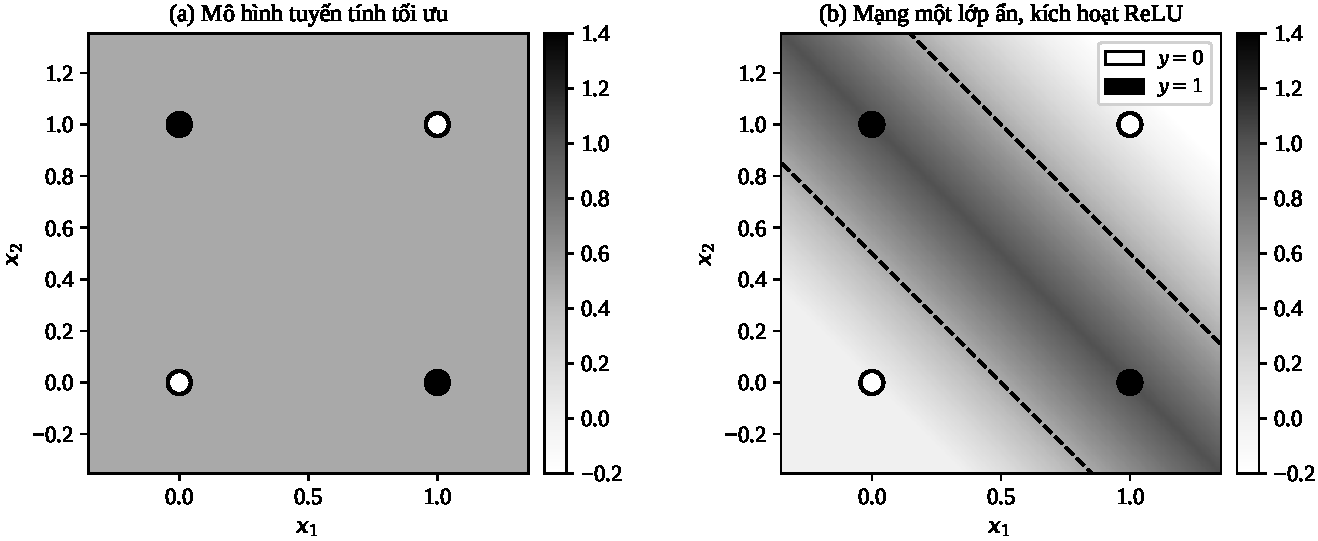
\includegraphics[width=0.95\textwidth]{Images/chap_2/hinh_xor.pdf}
\caption{Bài toán XOR. Điểm trắng ứng với $y=0$, điểm đen ứng với $y=1$; đường
đứt nét là mức $f = 0{,}5$. (a) Mô hình affine tối ưu là hằng số $0{,}5$ trên
toàn miền (Mệnh đề~\ref{md:xor-chan-duoi}), không có đường mức nào tách được dữ
liệu. (b) Mạng một lớp ẩn với tham số \eqref{eq:xor-net} tạo ra một dải giá trị
cao dọc theo đường $x_1+x_2=1$, tách đúng hai lớp.}
\label{fig:xor}
\end{figure}
 
\begin{nhanxet}
Hai điểm cần phân biệt rõ, cả hai đều sẽ tái xuất trong phần thực nghiệm.
 
Thứ nhất, Mệnh đề~\ref{md:xor-nghiem} chứng minh sự \emph{tồn tại} của bộ tham
số nghiệm, chứ không chứng minh rằng thuật toán tối ưu sẽ tìm được nó. Đây là
ranh giới giữa \emph{lý thuyết xấp xỉ} (khả năng biểu diễn) và \emph{lý thuyết
tối ưu} (khả năng học); ranh giới ấy được củng cố bởi
Mệnh đề~\ref{md:khong-loi} về tính không lồi.
 
Thứ hai, ví dụ này dùng ReLU và dùng tốt, trong khi Mục~\ref{sec:kichhoat} sẽ
loại trừ ReLU khỏi bài toán phương trình vi phân. Không có mâu thuẫn: ở đây ta
chỉ cần \emph{giá trị} của mạng khớp bốn nhãn, còn ở đó ta cần \emph{đạo hàm bậc
hai} của mạng khớp một phương trình. Tiêu chuẩn chọn hàm kích hoạt phụ thuộc vào
đại lượng nào của mạng được đưa vào hàm mục tiêu.
\end{nhanxet}
 
\subsection{Khả năng xấp xỉ phổ quát}
\label{subsec:xap-xi}
 
Ba định lý dưới đây trả lời ba câu hỏi khác nhau và thường bị gộp làm một trong
tài liệu phổ thông: mạng nơ-ron xấp xỉ được lớp hàm nào; xấp xỉ được theo
\emph{chuẩn} nào; và xấp xỉ với \emph{tốc độ} nào. Chỉ câu hỏi thứ hai và thứ ba
mới thực sự phục vụ báo cáo.
 
\begin{dinhly}[Xấp xỉ phổ quát, dạng $C^0$]
\label{dl:xap-xi}
Cho $K \subset \R^{d}$ compact và $\sigma \in C(\R)$ bị chặn địa phương. Tập các
hàm dạng
\begin{equation}
\Net(\bx) = \sum_{j=1}^{m} w_j\, \sigma\!\left( \bm{v}_j^{\top}\bx + c_j
\right),
\qquad m \in \mathbb{N}^{*},\ w_j, c_j \in \R,\ \bm{v}_j \in \R^{d},
\label{eq:xapxi}
\end{equation}
trù mật trong $C(K)$ với chuẩn hội tụ đều \emph{khi và chỉ khi} $\sigma$ không
phải là đa thức.
\end{dinhly}
 
\begin{nhanxet}[Về quy kết của Định lý~\ref{dl:xap-xi}]
\label{nx:quy-ket}
Dạng ``khi và chỉ khi $\sigma$ không phải đa thức'' ở trên là kết quả của Leshno
và cộng sự~\cite{leshno1993}, không phải của Cybenko hay Hornik. Cybenko
(\cite{cybenko1989}) chứng minh chiều thuận cho lớp hẹp hơn gồm các $\sigma$
\emph{sigmoidal}, tức liên tục với $\sigma(t)\to 1$ khi $t\to+\infty$ và
$\sigma(t)\to 0$ khi $t\to-\infty$. Việc phân biệt hai phát biểu là cần thiết
cho báo cáo: hàm $\sigma(t) = \sin t$ dùng trong một số kiến trúc PINN không
sigmoidal, nên chỉ nằm trong phạm vi của~\cite{leshno1993}. Chiều đảo của
Định lý~\ref{dl:xap-xi} chính là Mệnh đề~\ref{md:da-thuc} dưới đây, được chứng
minh đầy đủ vì lập luận sơ cấp và trực tiếp phục vụ tiêu chuẩn chọn $\sigma$.
\end{nhanxet}
 
\begin{proof}[Phác thảo chứng minh chiều thuận, theo Cybenko]
Ký hiệu $\mathcal{S}$ là bao đóng trong $C(K)$ của không gian sinh bởi các hàm
dạng \eqref{eq:xapxi}. Giả sử phản chứng $\mathcal{S} \ne C(K)$. Vì
$\mathcal{S}$ là không gian con đóng thực sự, theo định lý Hahn--Banach tồn tại
phiếm hàm tuyến tính liên tục $\Lambda \ne 0$ trên $C(K)$ triệt tiêu trên
$\mathcal{S}$. Theo định lý biểu diễn Riesz, tồn tại độ đo Borel chính quy hữu
hạn có dấu $\mu \ne 0$ sao cho $\Lambda(f) = \int_K f\,d\mu$. Khi đó
\[
\int_K \sigma(\bm{v}^{\top}\bx + c)\, d\mu(\bx) = 0
\qquad \forall\, \bm{v} \in \R^d,\ c \in \R .
\]
Bước then chốt là chứng minh rằng $\sigma$ trong lớp đang xét là \emph{phân
biệt} (discriminatory), tức đẳng thức trên buộc $\mu = 0$ -- mâu thuẫn. Ý tưởng:
dùng giả thiết về $\sigma$ để trích ra, qua phép lấy giới hạn khi tham số co
giãn tiến ra vô cùng, một hàm bậc thang; từ đó suy ra $\mu$ triệt tiêu trên mọi
nửa không gian, rồi kết luận bằng tính đầy đủ của hệ đặc trưng Fourier
$\bx\mapsto e^{i\bm{v}^{\top}\bx}$. Chi tiết đầy đủ xem~\cite{cybenko1989}; bản
sắc bén cho lớp không đa thức xem~\cite{leshno1993}.
\end{proof}
 
Đối với báo cáo này, dạng $C^0$ ở Định lý~\ref{dl:xap-xi} là \emph{chưa đủ}: nó
chỉ bảo đảm xấp xỉ giá trị hàm, không nói gì về đạo hàm. Một dãy hàm có thể hội
tụ đều tới $u$ trong khi đạo hàm của nó phân kỳ hoàn toàn; mà phần dư của phương
trình vi phân lại được xây trên đạo hàm. Dạng cần thiết là kết quả sau.
 
\begin{dinhly}[Hornik: xấp xỉ đồng thời đạo hàm]
\label{dl:sobolev}
Cho $K \subset \R^d$ compact, $k \in \mathbb{N}^{*}$, và $\sigma \in C^{k}(\R)$
không phải đa thức, với các đạo hàm tới bậc $k$ bị chặn. Khi đó tập các hàm dạng
\eqref{eq:xapxi} trù mật trong $C^{k}(K)$ theo chuẩn
\begin{equation}
\|f\|_{C^k(K)} = \max_{|\alpha| \le k}\ \sup_{\bx \in K}
  \big| \partial^{\alpha} f(\bx) \big| ,
\label{eq:chuan-ck}
\end{equation}
tức với mọi $f \in C^k(K)$ và $\varepsilon > 0$ tồn tại $\Net$ dạng
\eqref{eq:xapxi} sao cho $\|f - \Net\|_{C^k(K)} < \varepsilon$. Nói riêng, tập
ấy cũng trù mật trong không gian Sobolev $W^{k,\infty}(K)$.
\end{dinhly}
 
Định lý~\ref{dl:sobolev} (\cite{hornik1991}) là mệnh đề bảo đảm nền tảng cho
toàn bộ phương pháp: nếu nghiệm đúng $u$ của một phương trình vi phân bậc $k$
thuộc $C^k(K)$, thì tồn tại mạng nơ-ron làm nhỏ tuỳ ý cả sai số nghiệm lẫn sai
số của mọi đạo hàm tới bậc $k$, do đó làm nhỏ tuỳ ý phần dư. Hai điều kiện của
định lý đều mang tính bắt buộc và đều dẫn thẳng sang Mục~\ref{sec:kichhoat}:
$\sigma$ phải \emph{thuộc lớp $C^k$} và phải \emph{không là đa thức}.
 
Cần nhấn mạnh giới hạn của kết quả này. Nó khẳng định sự \emph{tồn tại} của một
bộ tham số tốt; nó không cho biết cần bao nhiêu nơ-ron, cũng không cho biết
thuật toán tối ưu có tìm được bộ tham số ấy hay không. Câu hỏi thứ nhất được
định lượng một phần bởi định lý sau; câu hỏi thứ hai vẫn để ngỏ trong toàn bộ
lĩnh vực.
 
\begin{dinhly}[Barron: tốc độ xấp xỉ]
\label{dl:barron}
Giả sử $f : \R^d \to \R$ có biến đổi Fourier $\hat f$ thoả mãn
\begin{equation}
C_f := \int_{\R^d} \|\bm{\omega}\|\,\big|\hat f(\bm{\omega})\big|\,
  d\bm{\omega} < \infty .
\label{eq:barron-hang-so}
\end{equation}
Khi đó với mọi $m \in \mathbb{N}^{*}$, tồn tại mạng một lớp ẩn $\Net_m$ với $m$
nơ-ron sigmoidal sao cho
\begin{equation}
\int_{K} \big( f(\bx) - \Net_m(\bx) \big)^2 \mu(d\bx)
 \;\le\; \frac{(2 r C_f)^2}{m},
\label{eq:barron}
\end{equation}
với $K$ là quả cầu bán kính $r$ và $\mu$ là độ đo xác suất tuỳ ý trên $K$.
\end{dinhly}
 
\begin{nhanxet}[Vì sao mạng nơ-ron hấp dẫn với bài toán nhiều chiều]
\label{nx:loi-nguyen}
Chặn \eqref{eq:barron} (\cite{barron1993}) có bậc $\mathcal{O}(m^{-1/2})$
\emph{không phụ thuộc số chiều $d$}; số chiều chỉ ẩn trong hằng số $C_f$. Trái
lại, các phương pháp xấp xỉ tuyến tính cổ điển -- đa thức, phần tử hữu hạn, lưới
sai phân -- trên lớp hàm trơn bậc $s$ chỉ đạt bậc $\mathcal{O}(m^{-s/d})$, suy
giảm nhanh khi $d$ tăng; đó là ``lời nguyền số chiều''. Đây là lập luận định
lượng chính biện minh cho việc dùng mạng nơ-ron thay cho lưới trong các bài toán
phương trình vi phân nhiều chiều.
 
Hai điều kiện phải đọc kèm. Thứ nhất, sự chuyển dịch phụ thuộc chiều từ
\emph{bậc} sang \emph{hằng số} không phải là sự biến mất của nó: với nhiều lớp
hàm, $C_f$ tự nó tăng theo $d$. Thứ hai, \eqref{eq:barron} là chặn theo chuẩn
$L^2$ chứ không phải chuẩn $C^k$ của Định lý~\ref{dl:sobolev}; không có kết quả
nào trong báo cáo cho phép ghép trực tiếp tốc độ của Barron với chuẩn cần thiết
cho phần dư. Ta dẫn Định lý~\ref{dl:barron} như một lập luận \emph{định hướng},
không như một chặn sai số áp dụng được cho các thí nghiệm ở
Chương~\ref{chap:thucnghiem}.
\end{nhanxet}
 
%==============================================================================
\section{Hàm kích hoạt}
\label{sec:kichhoat}
%==============================================================================
 
\subsection{Bốn điều kiện và nguồn gốc của chúng}
\label{subsec:yeu-cau}
 
Trong tài liệu học sâu, việc chọn hàm kích hoạt thường được trình bày như một
vấn đề kinh nghiệm --- xem chẳng hạn Mục 6.2.2 của Goodfellow và cộng
sự~\cite{goodfellow2016} hay phần khảo sát hàm kích hoạt
của Hammad~\cite{hammad2024}, nơi các hàm được so sánh chủ yếu theo hiệu quả
huấn luyện. Trong bài toán phương trình vi phân, phần lớn lựa chọn bị
ràng buộc bởi các kết quả đã thiết lập ở Mục~\ref{sec:cautruc}. Tổng hợp Hệ
quả~\ref{hq:suy-bien}, Hệ quả~\ref{hq:relu-hessian} và Định lý~\ref{dl:sobolev},
hàm kích hoạt $\sigma$ cần thoả mãn:
 
\begin{enumerate}[label=(\roman*), leftmargin=*]
\item \textbf{Không affine} -- điều kiện cần để mạng không suy biến thành ánh xạ
      affine (Hệ quả~\ref{hq:suy-bien}).
\item \textbf{Không đa thức} -- điều kiện cần và đủ cho tính trù mật
      (Định lý~\ref{dl:xap-xi}; chiều cần được chứng minh ở
      Mệnh đề~\ref{md:da-thuc}).
\item \textbf{Thuộc lớp $C^{k}$ với $k$ bằng bậc cao nhất của toán tử vi phân},
      và $\sigma^{(k)} \not\equiv 0$ (Hệ quả~\ref{hq:relu-hessian} và
      Nhận xét~\ref{nx:bac-cao}).
\item \textbf{Hành vi gradient lành mạnh} -- tích các $\sigma'$ dọc theo chiều
      sâu không được suy giảm hay bùng nổ quá nhanh
      (Mệnh đề~\ref{md:tich-gradient}).
\end{enumerate}
 
Ba điều kiện đầu là điều kiện \emph{cần} theo nghĩa toán học chặt chẽ: vi phạm
một trong ba thì phương pháp hỏng, không phải hoạt động kém. Điều kiện (iv) có
tính chất khác, là một yêu cầu định lượng về thang số và có thể được bù đắp một
phần bằng khởi tạo (Mục~\ref{sec:khoitao}).
 
\begin{menhde}[Hàm kích hoạt đa thức là không đủ]
\label{md:da-thuc}
Nếu $\sigma$ là đa thức bậc $p \ge 1$ thì mọi mạng theo
Định nghĩa~\ref{def:fnn} với $L$ lớp biểu diễn một đa thức bậc không quá
$p^{\,L-1}$. Do đó tập các hàm biểu diễn được nằm trong một không gian vectơ
hữu hạn chiều, là tập đóng và thực sự con của $C(K)$; nói riêng nó \emph{không}
trù mật trong $C(K)$.
\end{menhde}
 
\begin{proof}
Ta chứng minh bằng quy nạp rằng mỗi thành phần của $\ba^{(\ell)}$ là đa thức
theo $\bx$ với bậc không quá $p^{\ell}$.
 
Cơ sở $\ell = 0$: $\ba^{(0)} = \bx$ có bậc $1 = p^{0}$.
 
Bước quy nạp: theo \eqref{eq:z-k}, $z^{(\ell)}_k$ là tổ hợp tuyến tính của các
thành phần $a^{(\ell-1)}_j$ cộng hằng số, nên có bậc không quá $p^{\ell-1}$; hợp
thành với đa thức $\sigma$ bậc $p$ cho $a^{(\ell)}_k = \sigma(z^{(\ell)}_k)$ bậc
không quá $p\cdot p^{\ell-1} = p^{\ell}$.
 
Lớp ra là tổ hợp tuyến tính của $\ba^{(L-1)}$ nên $\Net_{\btheta}$ có bậc không
quá $p^{\,L-1}$.
 
Không gian các đa thức $d$ biến bậc không quá $D := p^{L-1}$ có số chiều
$\binom{D+d}{d} < \infty$. Mọi không gian con hữu hạn chiều của một không gian
định chuẩn đều đóng, và nó thực sự con vì $C(K)$ chứa các hàm không đa thức
(chẳng hạn $e^{x_1}$, với $K$ có phần trong khác rỗng). Vậy bao đóng của nó
không thể bằng $C(K)$.
\end{proof}
 
Điểm đáng chú ý: chặn $p^{L-1}$ tăng rất nhanh theo $L$, nên một mạng đa thức
sâu vẫn biểu diễn được các đa thức bậc rất cao. Sự thất bại ở đây không phải là
thất bại về \emph{dung lượng} mà về \emph{loại}: dù $L$ lớn đến đâu, lớp hàm thu
được vẫn nằm trong một không gian hữu hạn chiều đóng, và một hàm đơn giản như
$e^{x_1}$ mãi mãi nằm ngoài tầm với ở khoảng cách dương.
 
\subsection{Các hàm kích hoạt thông dụng}
 
\begin{table}[H]
\centering
\caption{So sánh các hàm kích hoạt thông dụng; $\sigma_{\mathrm{s}}$ ký hiệu
hàm sigmoid logistic. Cột cuối đối chiếu với điều kiện (iii) của
Mục~\ref{subsec:yeu-cau} cho toán tử bậc hai.}
\label{tab:kichhoat}
\small
\begin{tabular}{@{}l c c c c c@{}}
\toprule
\textbf{Tên} & \textbf{Biểu thức} & \textbf{Đạo hàm bậc nhất}
  & \textbf{Miền giá trị} & \textbf{Độ trơn} & $\sigma''\!\not\equiv\!0$ \\
\midrule
Sigmoid & $\dfrac{1}{1+e^{-z}}$
  & $\sigma_{\mathrm{s}}(1-\sigma_{\mathrm{s}})$ & $(0,1)$ & $C^{\infty}$
  & có \\[6pt]
Tanh & $\dfrac{e^{z}-e^{-z}}{e^{z}+e^{-z}}$
  & $1-\tanh^{2}z$ & $(-1,1)$ & $C^{\infty}$ & có \\[6pt]
ReLU & $\max\{0,z\}$
  & $\mathbf{1}_{\{z>0\}}$ & $[0,+\infty)$ & $C^{0}$ & \textbf{không} \\[6pt]
Leaky ReLU & $\max\{\alpha z, z\}$
  & $\mathbf{1}_{\{z>0\}} + \alpha\mathbf{1}_{\{z<0\}}$ & $\R$ & $C^{0}$
  & \textbf{không} \\[6pt]
Softplus & $\ln(1+e^{z})$
  & $\sigma_{\mathrm{s}}(z)$ & $(0,+\infty)$ & $C^{\infty}$ & có \\[6pt]
Swish (SiLU) & $z\,\sigma_{\mathrm{s}}(z)$
  & $\sigma_{\mathrm{s}} + z\sigma_{\mathrm{s}}(1-\sigma_{\mathrm{s}})$
  & $\approx[-0{,}28,+\infty)$ & $C^{\infty}$ & có \\[6pt]
Sine & $\sin z$ & $\cos z$ & $[-1,1]$ & $C^{\infty}$ & có \\
\bottomrule
\end{tabular}
\end{table}
 
\begin{figure}[H]
\centering
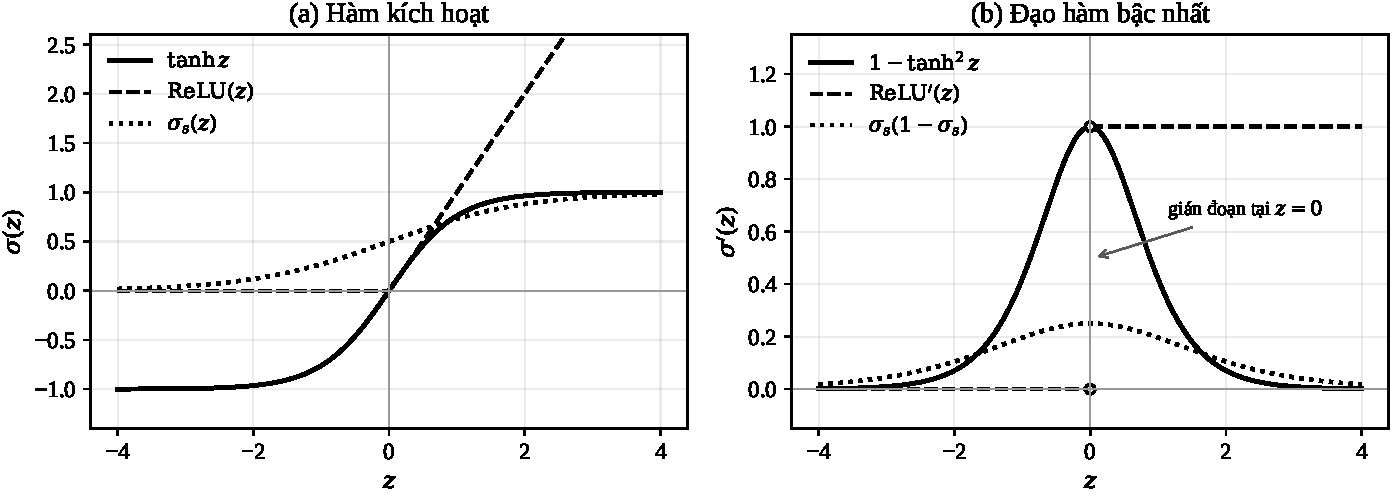
\includegraphics[width=0.98\textwidth]{Images/chap_2/hinh_kichhoat.pdf}
\caption{(a) Đồ thị ba hàm kích hoạt tiêu biểu. (b) Đạo hàm bậc nhất tương ứng.
Điểm gãy của ReLU tại $z=0$ thể hiện thành bước nhảy đơn vị của
$\mathrm{ReLU}'$. Đồng thời có thể thấy $\tanh'$ và $\sigma_{\mathrm{s}}'$ đều
tắt nhanh khi $|z| \gtrsim 3$, minh hoạ hiện tượng bão hoà được lượng hoá ở
Mệnh đề~\ref{md:tich-gradient}.}
\label{fig:kichhoat}
\end{figure}
 
\subsection{Giải tích của hàm tanh}
\label{subsec:tanh}
 
Vì $\tanh$ là hàm kích hoạt được chọn cho toàn bộ phần thực nghiệm, mục này
thiết lập ba tính chất của nó mà các chương sau sẽ dùng: cấu trúc đại số của đạo
hàm bậc cao, chặn đều cho mọi đạo hàm, và tốc độ tăng của đạo hàm tại gốc.
 
\begin{bode}[Cấu trúc đa thức của đạo hàm bậc cao]
\label{bd:tanh-dao-ham}
Đặt $\sigma(z) = \tanh z$. Tồn tại dãy đa thức $\{P_k\}_{k\ge 0}$ một biến sao
cho
\begin{equation}
\sigma^{(k)}(z) = P_k\big(\sigma(z)\big), \qquad k \ge 0,
\label{eq:tanh-Pk}
\end{equation}
xác định bởi $P_0(t) = t$ và hệ thức truy hồi
\begin{equation}
P_{k+1}(t) = \big(1 - t^2\big)\, P_k'(t).
\label{eq:tanh-truy-hoi}
\end{equation}
Hơn nữa $\deg P_k = k+1$ với mọi $k \ge 0$.
\end{bode}
 
\begin{proof}
Với $k = 0$, \eqref{eq:tanh-Pk} là định nghĩa của $P_0$. Giả sử
$\sigma^{(k)} = P_k \circ \sigma$. Lấy đạo hàm và dùng
$\sigma' = 1 - \sigma^2$ (suy trực tiếp từ
$\tanh' = \sech^2 = 1 - \tanh^2$):
\[
\sigma^{(k+1)}(z) = P_k'\big(\sigma(z)\big)\,\sigma'(z)
 = P_k'\big(\sigma(z)\big)\big(1 - \sigma(z)^2\big)
 = P_{k+1}\big(\sigma(z)\big),
\]
với $P_{k+1}$ cho bởi \eqref{eq:tanh-truy-hoi}.
 
Về bậc: $\deg P_0 = 1$ với hệ số dẫn đầu $c_0 = 1$. Nếu $\deg P_k = k+1$ với hệ
số dẫn đầu $c_k \ne 0$ thì $\deg P_k' = k$ với hệ số dẫn đầu $(k+1)c_k$, và nhân
với $(1-t^2)$ cho $\deg P_{k+1} = k+2$ với hệ số dẫn đầu $-(k+1)c_k \ne 0$. Quy
nạp kết thúc.
\end{proof}
 
Ba phần tử đầu của dãy, thu được bằng cách áp dụng
\eqref{eq:tanh-truy-hoi} hai lần:
\begin{align}
\sigma'(z)   &= 1 - \sigma^{2}, \label{eq:tanh-d1}\\
\sigma''(z)  &= -2\sigma\left(1-\sigma^{2}\right)
             = -2\sigma + 2\sigma^3, \label{eq:tanh-d2}\\
\sigma'''(z) &= -2\left(1-\sigma^{2}\right)\left(1-3\sigma^{2}\right)
             = -2 + 8\sigma^2 - 6\sigma^4. \label{eq:tanh-d3}
\end{align}
Công thức \eqref{eq:tanh-d2} là công thức được dùng ở Ví dụ~\ref{vd:dao-ham} và
ở dòng 6 của Thuật toán~\ref{alg:dao-ham}. Điểm thực hành đáng lưu ý: nhờ
\eqref{eq:tanh-Pk}, mọi đạo hàm bậc cao của $\tanh$ được tính \emph{chỉ từ giá
trị $\tanh z$ đã có}, không cần đánh giá lại hàm mũ.
 
\begin{hequa}[Chặn đều cho mọi đạo hàm]
\label{hq:tanh-chan}
Với mọi $k \ge 0$,
\begin{equation}
\sup_{z\in\R} \big|\sigma^{(k)}(z)\big|
 \;\le\; \max_{|t| \le 1} \big|P_k(t)\big| =: M_k < \infty .
\label{eq:tanh-chan}
\end{equation}
Cụ thể $M_0 = 1$, $M_1 = 1$, $M_2 = \dfrac{4}{3\sqrt{3}} \approx 0{,}7698$.
\end{hequa}
 
\begin{proof}
Vì $\sigma(\R) = (-1,1) \subset [-1,1]$, kết hợp \eqref{eq:tanh-Pk} với tính
liên tục của $P_k$ trên compact $[-1,1]$ cho \eqref{eq:tanh-chan}. Giá trị
$M_0 = \max_{|t|\le1}|t| = 1$. Giá trị $M_1 = \max_{|t|\le1}|1-t^2| = 1$, đạt
tại $t = 0$. Giá trị $M_2$: xét $h(t) = -2t + 2t^3$ trên $[-1,1]$; ta có
$h'(t) = -2 + 6t^2 = 0$ tại $t = \pm 1/\sqrt3$, cho
$|h| = 2/\sqrt3 - 2/(3\sqrt3) = 4/(3\sqrt3)$, còn tại hai đầu mút $h(\pm1) = 0$.
\end{proof}
 
Hệ quả~\ref{hq:tanh-chan} có ý nghĩa thực hành trực tiếp: nó cho phép chặn đều
mọi số hạng chứa $\sigma^{(m)}$ trong hệ truy hồi \eqref{eq:S-truy-hoi}, bảo đảm
rằng đạo hàm bậc cao của mạng $\tanh$ \emph{không thể} bùng nổ do bản thân hàm
kích hoạt. Nếu $\nabla^2_{\bx}\Net_{\btheta}$ bùng nổ trong thực nghiệm, nguyên
nhân chỉ có thể là trọng số lớn -- tức là vấn đề khởi tạo hoặc vấn đề tối ưu,
không phải vấn đề kiến trúc. Đây là một tiêu chuẩn chẩn đoán hữu ích khi gỡ lỗi
huấn luyện.
 
\begin{menhde}[Tính giải tích và bán kính hội tụ]
\label{md:tanh-giai-tich}
Hàm $\tanh$ chỉnh hình trên dải
$\{z \in \mathbb{C} : |\operatorname{Im} z| < \pi/2\}$ và có cực điểm đơn tại
$z = \pm i\pi/2$. Do đó chuỗi Taylor của $\tanh$ tại $0$ có bán kính hội tụ đúng
bằng $\pi/2$, và
\begin{equation}
\limsup_{k\to\infty}
  \left(\frac{\big|\sigma^{(k)}(0)\big|}{k!}\right)^{\!1/k}
 = \frac{2}{\pi},
\qquad\text{tức}\qquad
\forall\,\epsilon>0\ \ \exists\, C_\epsilon:\;
\big|\sigma^{(k)}(0)\big| \le C_\epsilon\, k!
  \left(\frac{2}{\pi}+\epsilon\right)^{\!k} .
\label{eq:tanh-tang}
\end{equation}
\end{menhde}
 
\begin{proof}
$\tanh z = \sinh z/\cosh z$ là thương của hai hàm nguyên; các điểm kỳ dị là
nghiệm của $\cosh z = 0$, tức $z = i\pi/2 + ik\pi$, $k \in \mathbb{Z}$. Điểm kỳ
dị gần gốc nhất cách gốc $\pi/2$, nên bán kính hội tụ bằng $\pi/2$. Đẳng thức
\eqref{eq:tanh-tang} chính là công thức Cauchy--Hadamard áp cho hệ số Taylor
$a_k = \sigma^{(k)}(0)/k!$: bán kính hội tụ $R = \big(\limsup_k
|a_k|^{1/k}\big)^{-1}$ bằng $\pi/2$. Dạng thứ hai suy ra từ định nghĩa của
$\limsup$.
\end{proof}
 
\begin{nhanxet}[Vì sao không viết được chặn với đúng cơ số $2/\pi$]
Bất đẳng thức Cauchy cho $|a_k| \le M(r)/r^{k}$ với mọi $r < \pi/2$, trong đó
$M(r) = \max_{|z|=r}|\tanh z|$; nhưng $M(r) \to \infty$ khi $r \to \pi/2^{-}$ vì
$\tanh$ có cực tại $i\pi/2$, nên \emph{không} thể chọn $r = \pi/2$ để thu được
chặn dạng $|\sigma^{(k)}(0)| \le C\,k!\,(2/\pi)^k$ chỉ bằng lập luận này. Chặn
với đúng cơ số $2/\pi$ vẫn đúng, nhưng đòi hỏi khai triển thặng dư tại cực đơn
$i\pi/2$ chứ không phải bất đẳng thức Cauchy. Vì báo cáo chỉ cần \emph{bậc}
tăng, ta dừng ở \eqref{eq:tanh-tang}.
\end{nhanxet}
 
Mệnh đề~\ref{md:tanh-giai-tich} lý giải một quan sát thực nghiệm quen thuộc: vi
phân tự động bậc cao trên mạng $\tanh$ ổn định về số, vì các đạo hàm tại gốc chỉ
tăng theo cấp giai thừa với cơ số $2/\pi < 1$, chứ không nhanh hơn. Trong thực hành, các phương
trình được xét ở báo cáo này có bậc không quá $2$, nên chỉ cần
\eqref{eq:tanh-d1}--\eqref{eq:tanh-d2}.
 
\subsection{Cấu trúc của mạng ReLU}
\label{subsec:relu}
 
Mục này giải thích, bằng hai lối lập luận độc lập, vì sao ReLU -- lựa chọn mặc
định gần như tuyệt đối trong thị giác máy tính -- lại vắng bóng hoàn toàn trong
tài liệu về phương trình vi phân.
 
\begin{dinhly}[Mạng ReLU là hàm tuyến tính từng khúc]
\label{dl:relu-tuyen-tinh}
Với $\sigma = \mathrm{ReLU}$, tồn tại một họ hữu hạn các đa diện lồi
$\{\Omega_1,\dots,\Omega_R\}$ có phần trong rời nhau, phủ $\R^{n_0}$, sao cho
$\Net_{\btheta}$ trùng với một ánh xạ affine trên mỗi $\Omega_r$.
\end{dinhly}
 
\begin{proof}
Ta chứng minh bằng quy nạp theo $\ell$ rằng tồn tại phân hoạch đa diện hữu hạn
$\mathcal{P}^{(\ell)}$ của $\R^{n_0}$ sao cho $\ba^{(\ell)}$ là affine trên mỗi
ô.
 
Cơ sở $\ell = 0$: $\ba^{(0)} = \bx$ affine trên
$\mathcal{P}^{(0)} = \{\R^{n_0}\}$.
 
Bước quy nạp: trên mỗi ô $\Omega \in \mathcal{P}^{(\ell-1)}$, $\ba^{(\ell-1)}$
affine, nên $\bz^{(\ell)} = \bW^{(\ell)}\ba^{(\ell-1)} + \bb^{(\ell)}$ cũng
affine trên $\Omega$; viết $z^{(\ell)}_k(\bx) = \bm{\alpha}_k^{\top}\bx +
\beta_k$ trên $\Omega$. Chia $\Omega$ bởi $n_\ell$ siêu phẳng
$H_k = \{\bm{\alpha}_k^{\top}\bx + \beta_k = 0\}$ thành tối đa $2^{n_\ell}$ ô
con, mỗi ô con vẫn là đa diện lồi (giao của $\Omega$ với các nửa không gian).
Trên mỗi ô con, dấu của $z^{(\ell)}_k$ không đổi với mọi $k$, nên
$a^{(\ell)}_k = \max\{0, z^{(\ell)}_k\}$ bằng $z^{(\ell)}_k$ hoặc bằng $0$ --
trong cả hai trường hợp đều affine. Lấy $\mathcal{P}^{(\ell)}$ là họ tất cả các
ô con thu được; đó là họ hữu hạn vì $\mathcal{P}^{(\ell-1)}$ hữu hạn.
 
Cuối cùng, lớp ra là ánh xạ affine của $\ba^{(L-1)}$ nên $\Net_{\btheta}$ affine
trên mỗi ô của $\mathcal{P}^{(L-1)}$.
\end{proof}
 
\begin{hequa}[Hessian triệt tiêu hầu khắp nơi]
\label{hq:relu-hkn}
Với $\sigma = \mathrm{ReLU}$,
\begin{equation}
\nabla^2_{\bx} \Net_{\btheta}(\bx) = \bm{0}
\qquad \text{với hầu khắp } \bx \in \R^{n_0}
\ (\text{theo độ đo Lebesgue}).
\label{eq:relu-hessian-zero}
\end{equation}
\end{hequa}
 
\begin{proof}
Theo Định lý~\ref{dl:relu-tuyen-tinh}, $\Net_{\btheta}$ affine trên phần trong
của mỗi $\Omega_r$, nên Hessian triệt tiêu ở đó. Phần bù
$\R^{n_0}\setminus\bigcup_r \operatorname{int}\Omega_r$ chứa trong hợp hữu hạn
các siêu phẳng, là tập có độ đo Lebesgue bằng $0$.
\end{proof}
 
Kết luận \eqref{eq:relu-hessian-zero} cũng suy được từ Hệ
quả~\ref{hq:relu-hessian} bằng cách áp dụng nó tại mỗi $\bx$ nằm ngoài tập điểm
gãy, nơi $\sigma'' = 0$ trên một lân cận. Hai lối chứng minh soi sáng hai mặt
khác nhau của cùng một hiện tượng: một mặt hình học (phân hoạch đa diện), một
mặt giải tích (truy hồi độ cong). Mệnh đề sau cho biết ``phần độ cong bị mất''
đã đi đâu.
 
\begin{menhde}[Đạo hàm bậc hai theo nghĩa phân bố, trường hợp một chiều]
\label{md:dirac}
Xét $n_0 = n_L = 1$, $L = 2$, tức
$\Net(x) = \sum_{j=1}^{m} w_j\,\mathrm{ReLU}(v_j x + c_j) + b$ với
$v_j \ne 0$. Khi đó, theo nghĩa phân bố trên $\mathcal{D}'(\R)$,
\begin{equation}
\Net'' = \sum_{j=1}^{m} w_j\, |v_j|\; \delta_{x_j},
\qquad x_j := -\,c_j/v_j .
\label{eq:dirac}
\end{equation}
Nói riêng, $\Net''$ là một tổ hợp tuyến tính hữu hạn các độ đo Dirac, có giá là
tập hữu hạn $\{x_1,\dots,x_m\}$ có độ đo Lebesgue bằng $0$.
\end{menhde}
 
\begin{proof}
Đủ xét một số hạng $u(x) = \mathrm{ReLU}(vx+c)$. Vì $u$ liên tục và tuyến tính
từng khúc, đạo hàm phân bố của nó là
$u'(x) = v\,\mathbf{1}_{\{vx+c>0\}}$. Hàm chỉ báo này là hàm bậc thang với bước
nhảy tại $x_0 = -c/v$: nếu $v > 0$ thì $\{vx+c>0\} = (x_0,\infty)$ và chỉ báo
nhảy từ $0$ lên $1$; nếu $v<0$ thì $\{vx+c>0\} = (-\infty,x_0)$ và chỉ báo nhảy
từ $1$ xuống $0$. Trong cả hai trường hợp biên độ bước nhảy là
$\operatorname{sgn}(v)$. Đạo hàm phân bố của hàm bậc thang Heaviside là $\delta$,
nên
\[
u'' = v \cdot \operatorname{sgn}(v)\,\delta_{x_0} = |v|\,\delta_{x_0}.
\]
Lấy tổ hợp tuyến tính với hệ số $w_j$ và dùng tính tuyến tính của đạo hàm phân
bố cho \eqref{eq:dirac}.
\end{proof}
 
Cần đọc \eqref{eq:dirac} cho đúng: đạo hàm bậc hai của mạng ReLU không phải là
$0$; nó là một phân bố kỳ dị. Nhưng vi phân tự động không tính phân bố, nó tính
giá trị điểm; và tại hầu khắp mọi điểm, giá trị ấy bằng $0$. Chính khoảng cách
giữa hai khái niệm đạo hàm này sinh ra hệ quả sau.
 
\subsection{Hệ quả đối với bài toán phương trình vi phân}
 
\begin{hequa}[Sụp đổ của gradient huấn luyện với kiến trúc ReLU]
\label{hq:pinn-hong}
Xét bài toán $-u''(x) = f(x)$ trên $\Omega \subset \R$ và hàm mục tiêu phần dư
\begin{equation}
J(\btheta) = \frac{1}{N_r}\sum_{i=1}^{N_r}
  \Big( -\Net''_{\btheta}(x_i) - f(x_i) \Big)^{2}.
\label{eq:J-residual}
\end{equation}
Giả sử $\sigma = \mathrm{ReLU}$ và các điểm phối trí $x_i$ được lấy mẫu từ một
phân phối liên tục tuyệt đối trên $\Omega$. Khi đó, với xác suất $1$, tồn tại
lân cận $U$ của $\btheta$ trong $\R^P$ sao cho
\begin{equation}
J(\btheta') = \frac{1}{N_r}\sum_{i=1}^{N_r} f(x_i)^2
\quad \forall\, \btheta' \in U,
\qquad\text{và do đó}\qquad
\nabla_{\btheta} J(\btheta) = \bm{0}.
\label{eq:gradient-zero}
\end{equation}
\end{hequa}
 
\begin{proof}
Theo Định lý~\ref{dl:relu-tuyen-tinh}, phân hoạch $\mathcal{P}^{(L-1)}$ của
$\R$ là hữu hạn, nên tập điểm gãy $\mathcal{K}(\btheta)$ -- hợp các biên của các
ô -- là tập hữu hạn, do đó có độ đo Lebesgue $0$. Vì phân phối lấy mẫu liên tục
tuyệt đối, $\mathbb{P}\big(\exists\, i:\ x_i \in \mathcal{K}(\btheta)\big) = 0$.
Vậy với xác suất $1$, mọi $x_i$ đều nằm trong phần trong của một ô, nơi
$\Net''_{\btheta}(x_i) = 0$ theo Hệ quả~\ref{hq:relu-hkn}.
 
Hơn nữa, điều vừa nói tương đương với $z^{(\ell)}_k(x_i) \ne 0$ với mọi
$i,\ell,k$, vì các điểm gãy đúng là nơi một tiền kích hoạt đổi dấu. Mỗi hàm
$\btheta' \mapsto z^{(\ell)}_k(x_i)$ liên tục (hợp thành của các phép affine và
ReLU, đều liên tục), và bộ ba chỉ số $(i,\ell,k)$ chạy trên một tập
\emph{hữu hạn}. Vậy tồn tại lân cận $U$ của $\btheta$ mà trên đó cả hữu hạn
đại lượng ấy đều giữ nguyên dấu, nói riêng không triệt tiêu: không một điểm gãy
nào có thể rơi trúng một $x_i$ khi $\btheta'$ còn nằm trong $U$. Trên $U$ ta có
$\Net''_{\btheta'}(x_i) = 0$ với mọi $i$; thay vào \eqref{eq:J-residual} cho
$J$ hằng trên $U$ với giá trị nêu ở \eqref{eq:gradient-zero}. Một hàm hằng địa
phương có gradient bằng $0$.
\end{proof}
 
Hệ quả~\ref{hq:pinn-hong} phát biểu chính xác điều mà tài liệu thường chỉ mô tả
định tính. Điểm cần nhấn mạnh: đây \emph{không} phải hiện tượng ``hội tụ chậm''
hay ``khó tối ưu''. Hàm mục tiêu là \emph{hằng số địa phương}, nên mọi thuật
toán dựa trên gradient -- SGD, Adam, L-BFGS~\cite{nocedal2006} -- đều đứng yên
tuyệt đối tại mọi điểm khởi tạo. Mô hình nằm ngoài không gian hàm chứa nghiệm,
và không có cách tinh chỉnh siêu tham số nào cứu vãn được.
 
\begin{nhanxet}
Lập luận trên cũng giải thích vì sao các hàm kích hoạt trơn khác -- softplus,
Swish, sine -- vẫn được xem xét trong tài liệu về phương trình vi
phân~\cite{karniadakis2021}, trong khi ReLU thì không. Với phương trình bậc nhất
($\mathcal{L} = \partial_x$), ReLU về nguyên tắc dùng được vì $\Net'$ không đồng
nhất triệt tiêu; nhưng khi ấy $\Net'$ là hàm bậc thang, không thể xấp xỉ tốt một
đạo hàm liên tục theo chuẩn đều -- đúng như Định lý~\ref{dl:sobolev} dự báo, vì
ReLU không thuộc $C^1$.
\end{nhanxet}
 
\subsection{Bão hoà và triệt tiêu gradient}
\label{subsec:bao-hoa}
 
Ưu thế về độ trơn của $\tanh$ không miễn phí. Kết quả sau lượng hoá cái giá phải
trả, và là nội dung của điều kiện (iv) ở Mục~\ref{subsec:yeu-cau}.
 
\begin{menhde}[Chặn tích gradient theo chiều sâu]
\label{md:tich-gradient}
Đặt $\bm{\delta}^{(\ell)} = \partial J/\partial\bz^{(\ell)}$. Từ quy tắc dây
chuyền, $\bm{\delta}^{(\ell-1)} = \bD^{(\ell-1)}
\big(\bW^{(\ell)}\big)^{\!\top}\bm{\delta}^{(\ell)}$, và do đó
\begin{equation}
\big\|\bm{\delta}^{(1)}\big\|_2
 \;\le\; \big\|\bm{\delta}^{(L)}\big\|_2
   \prod_{\ell=2}^{L} \big\|\bW^{(\ell)}\big\|_2
   \prod_{\ell=1}^{L-1} \big\|\bD^{(\ell)}\big\|_2 .
\label{eq:chan-gradient}
\end{equation}
Với $\sigma = \tanh$ ta có
$\|\bD^{(\ell)}\|_2 = \max_k \big(1 - \tanh^2 z^{(\ell)}_k\big) \le 1$; nếu
ngoài ra $|z^{(\ell)}_k| \ge \tau$ với mọi $k,\ell$ thì
\begin{equation}
\big\|\bm{\delta}^{(1)}\big\|_2 \;\le\;
\big\|\bm{\delta}^{(L)}\big\|_2 \left(\prod_{\ell=2}^{L}
\big\|\bW^{(\ell)}\big\|_2\right)
\sech^{2(L-1)}(\tau),
\label{eq:chan-bao-hoa}
\end{equation}
tức thừa số do bão hoà đóng góp vào chặn trên suy giảm theo cấp số nhân với cơ
số $\sech^{2}(\tau) < 1$. Cần đọc \eqref{eq:chan-bao-hoa} cho đúng: đây là chặn
\emph{trên}, và nó chỉ kéo theo gradient thực sự triệt tiêu khi tích
$\prod_{\ell=2}^{L}\|\bW^{(\ell)}\|_2$ không bù lại được sự suy giảm ấy -- điều
được bảo đảm dưới khởi tạo Xavier (Mục~\ref{sec:khoitao}), nơi mỗi
$\|\bW^{(\ell)}\|_2$ ở thang $\mathcal{O}(1)$.
\end{menhde}
 
\begin{proof}
Hệ thức truy hồi cho $\bm{\delta}$ là quy tắc dây chuyền chuẩn, được dẫn chi
tiết ở Chương~\ref{chap:autodiff}. Bất đẳng thức \eqref{eq:chan-gradient} suy từ
tính nhân dưới của chuẩn phổ, $\|\bm{A}\bu\|_2 \le \|\bm{A}\|_2\|\bu\|_2$, áp
dụng lặp. Với $\bD$ đường chéo, $\|\bD\|_2$ bằng giá trị tuyệt đối lớn nhất trên
đường chéo, ở đây là $\max_k \sech^2 z^{(\ell)}_k$. Cuối cùng,
$1 - \tanh^2 t = \sech^2 t$ là hàm chẵn, giảm ngặt trên $[0,\infty)$, nên
$|z| \ge \tau$ kéo theo $\sech^2 z \le \sech^2 \tau$.
\end{proof}
 
Ví dụ số cho thấy mức độ nghiêm trọng (lấy
$\prod_{\ell}\|\bW^{(\ell)}\|_2 = 1$ để cô lập riêng ảnh hưởng của bão hoà): với
$\tau = 3$ ta có
$\sech^2(3) \approx 0{,}00987$; qua $L-1 = 10$ lớp bão hoà, hệ số suy giảm là
$0{,}00987^{10} \approx 8{,}7\times10^{-21}$ -- gradient bị triệt tiêu hoàn toàn
trong số học dấu phẩy động độ chính xác kép, nơi epsilon máy vào cỡ
$2{,}2\times10^{-16}$. Đây chính là lý do Mục~\ref{sec:khoitao} là bắt buộc chứ
không phải tuỳ chọn: phải giữ $|z^{(\ell)}|$ nhỏ ngay từ thời điểm khởi tạo, vì
một khi mạng đã bão hoà thì không còn tín hiệu gradient để thoát ra.
 
\subsection{Kiểm chứng số}
 
Thí nghiệm TN-B kiểm chứng \eqref{eq:tanh-d1}--\eqref{eq:tanh-d3} bằng sai phân
hữu hạn trung tâm tại năm điểm rải trên $[-2;\,3]$. Sai số tối đa thu được lần
lượt là $3{,}3\times10^{-9}$, $9{,}0\times10^{-9}$ và $4{,}4\times10^{-5}$ cho
đạo hàm bậc một, hai và ba -- hoàn toàn tương thích với bậc chính xác của các
lược đồ sai phân được dùng, trong đó lược đồ bậc ba nhạy cảm nhất với sai số làm
tròn do chia cho $h^3$.
 
Cùng thí nghiệm định lượng Hệ quả~\ref{hq:relu-hkn} trên lưới $501$ điểm với
mạng ReLU $H = 32$ nơ-ron: $97{,}8\%$ số điểm cho $|\Net''_{\btheta}| < 1$ với
giá trị cực đại chỉ $5{,}0\times10^{-10}$, đúng bằng mức sai số làm tròn của
lược đồ sai phân; $11$ điểm còn lại nằm sát các điểm gãy và cho giá trị bùng nổ.
Đây là biểu hiện số của các độ đo Dirac trong \eqref{eq:dirac}: sai phân hữu hạn
với bước $h$ ``nhìn thấy'' một Dirac dưới dạng một xung biên độ
$\mathcal{O}(1/h)$ khi điểm lưới rơi gần điểm gãy.
 
%==============================================================================
\section{Khởi tạo trọng số và độ chệch}
\label{sec:khoitao}
%==============================================================================
 
Mục~\ref{sec:kichhoat} kết luận rằng phải giữ $|z^{(\ell)}|$ nhỏ tại thời điểm
bắt đầu huấn luyện. Mục này biến yêu cầu định tính ấy thành một công thức cho
phương sai của trọng số khởi tạo, qua ba bước: loại trừ khởi tạo hằng
(Mục~\ref{subsec:doi-xung}), thiết lập điều kiện bảo toàn phương sai
(Mục~\ref{subsec:phuong-sai}), và hiệu chỉnh sai lệch bậc hai giữa lý thuyết và
thực nghiệm (Mục~\ref{subsec:hieu-chinh}).
 
\subsection{Phá vỡ đối xứng}
\label{subsec:doi-xung}
 
\begin{menhde}[Khởi tạo hằng làm suy biến bề rộng]
\label{md:doi-xung}
Giả sử tại thời điểm khởi tạo, với mỗi $\ell$ tồn tại các hằng số
$c_\ell, d_\ell \in \R$ sao cho
\begin{equation}
w^{(\ell)}_{kj} = c_\ell \ \ \forall k,j,
\qquad
b^{(\ell)}_k = d_\ell \ \ \forall k .
\label{eq:khoi-tao-hang}
\end{equation}
Khi huấn luyện bằng gradient descent toàn phần, tính chất
\eqref{eq:khoi-tao-hang} được bảo toàn qua mọi bước lặp. Nói riêng, mọi nơ-ron
trong cùng một lớp luôn có cùng kích hoạt và cùng gradient, nên lớp $\ell$ hành
xử như lớp chỉ có một nơ-ron, bất kể $n_\ell$ lớn đến đâu. Trường hợp riêng
$c_\ell = d_\ell = 0$ là khởi tạo bằng không.
\end{menhde}
 
\begin{proof}
Quy nạp theo số bước lặp. Giả sử \eqref{eq:khoi-tao-hang} đúng với mọi $\ell$
tại bước hiện tại; ta chứng minh nó vẫn đúng sau một bước cập nhật.
 
\emph{Bước 1: kích hoạt hằng theo thành phần.} Từ \eqref{eq:z-k},
$z^{(1)}_k = c_1\sum_j x_j + d_1$ không phụ thuộc $k$, nên các thành phần của
$\ba^{(1)}$ bằng nhau. Quy nạp theo $\ell$: nếu các thành phần của
$\ba^{(\ell-1)}$ bằng nhau, ký hiệu chung là $\bar a^{(\ell-1)}$, thì
$z^{(\ell)}_k = c_\ell\, n_{\ell-1}\, \bar a^{(\ell-1)} + d_\ell$ không phụ
thuộc $k$. Vậy mọi $\ba^{(\ell)}$ đều có các thành phần bằng nhau, và ta ký hiệu
$\bar z^{(\ell)}, \bar a^{(\ell)}$ cho giá trị chung.
 
\emph{Bước 2: sai số ngược hằng theo thành phần.} Ta chứng minh quy nạp lùi rằng
các thành phần của $\bm{\delta}^{(\ell)}$ bằng nhau. Tại lớp ra, điều này hiển
nhiên khi $n_L = 1$; với $n_L > 1$ nó đúng khi hàm mất mát đối xứng theo các
thành phần đầu ra, điều thoả mãn với MSE. Giả sử các thành phần của
$\bm{\delta}^{(\ell+1)}$ bằng nhau và bằng $\bar\delta^{(\ell+1)}$. Từ
$\bm{\delta}^{(\ell)} = \bD^{(\ell)}\big(\bW^{(\ell+1)}\big)^{\!\top}
\bm{\delta}^{(\ell+1)}$, thành phần thứ $k$ là
\[
\delta^{(\ell)}_k
 = \sigma'\!\big(\bar z^{(\ell)}\big)
   \sum_{i=1}^{n_{\ell+1}} w^{(\ell+1)}_{ik}\,\delta^{(\ell+1)}_i
 = \sigma'\!\big(\bar z^{(\ell)}\big)\, c_{\ell+1}\, n_{\ell+1}\,
   \bar\delta^{(\ell+1)},
\]
không phụ thuộc $k$. Ở đây ta đã dùng \emph{đầy đủ} giả thiết
\eqref{eq:khoi-tao-hang}: $w^{(\ell+1)}_{ik} = c_{\ell+1}$ với mọi cặp chỉ số.
 
\emph{Bước 3: gradient là ma trận hằng.} Ta có
$\partial J/\partial w^{(\ell)}_{kj} = \delta^{(\ell)}_k\, a^{(\ell-1)}_j
 = \bar\delta^{(\ell)}\,\bar a^{(\ell-1)}$, không phụ thuộc cả $k$ lẫn $j$;
tương tự $\partial J/\partial b^{(\ell)}_k = \bar\delta^{(\ell)}$ không phụ
thuộc $k$. Vậy bước cập nhật
$\bW^{(\ell)} \gets \bW^{(\ell)} - \eta\,\partial J/\partial\bW^{(\ell)}$ trừ đi
cùng một số khỏi mọi phần tử, nên \eqref{eq:khoi-tao-hang} được bảo toàn với các
hằng số mới. Lập luận tương tự cho $\bb^{(\ell)}$.
\end{proof}
 
\begin{nhanxet}[Về một giả thiết yếu hơn và không đủ]
\label{nx:phan-vi-du}
Trong tài liệu, mệnh đề trên đôi khi được phát biểu với giả thiết yếu hơn: ``mọi
\emph{hàng} của $\bW^{(\ell)}$ bằng nhau''. Giả thiết ấy đủ cho Bước 1 nhưng
\emph{không} được bảo toàn qua bước cập nhật, nên phát biểu đó không đúng. Thật
vậy, nếu $\bW^{(\ell+1)}$ chỉ có các hàng bằng nhau, tức
$w^{(\ell+1)}_{ik} = \omega_k$ phụ thuộc $k$, thì Bước 2 cho
\[
\delta^{(\ell)}_k
 = \sigma'\!\big(\bar z^{(\ell)}\big)\,\omega_k
   \sum_{i} \delta^{(\ell+1)}_i
 = C\,\omega_k ,
\]
phụ thuộc $k$. Khi đó hàng thứ $k$ của ma trận gradient bằng
$C\,\omega_k\,\big(\ba^{(\ell-1)}\big)^{\!\top}$: các hàng chỉ \emph{tỉ lệ} với
nhau chứ không bằng nhau, và sau một bước cập nhật tính chất ``các hàng bằng
nhau'' bị phá vỡ. Nói cách khác, đối xứng thực sự được bảo toàn là đối xứng
\emph{hoán vị đầy đủ} giữa các nơ-ron trong một lớp, mà \eqref{eq:khoi-tao-hang}
là điều kiện đủ tự nhiên nhất để có nó.
\end{nhanxet}
 
Mệnh đề~\ref{md:doi-xung} loại trừ khởi tạo hằng: trọng số phải được khởi tạo
\emph{ngẫu nhiên}. Câu hỏi còn lại là với phương sai bằng bao nhiêu.
 
\subsection{Phân tích lan truyền phương sai}
\label{subsec:phuong-sai}
 
\begin{bode}[Phương sai của tổ hợp tuyến tính ngẫu nhiên]
\label{bd:phuong-sai}
Cho $W_1,\dots,W_n$ độc lập cùng phân phối với $\E W_j = 0$, $\Var W_j = v$, và
$a_1,\dots,a_n$ độc lập với $\{W_j\}$ và có $\E[a_j^2] < \infty$. Đặt
$z = \sum_{j=1}^{n} W_j a_j$. Khi đó
\begin{equation}
\E[z] = 0, \qquad
\Var(z) = \E[z^2] = v \sum_{j=1}^{n} \E\big[a_j^2\big]
        = n\, v\, \E\big[a^2\big]
\label{eq:bo-de-var}
\end{equation}
(đẳng thức cuối khi các $a_j$ cùng phân phối).
\end{bode}
 
\begin{proof}
Do độc lập, $\E[z] = \sum_j \E[W_j]\,\E[a_j] = 0$. Tiếp theo
\[
\E[z^2] = \sum_{j}\sum_{k} \E\big[W_j W_k a_j a_k\big]
        = \sum_{j}\sum_{k} \E\big[W_j W_k\big]\, \E\big[a_j a_k\big],
\]
trong đó bước thứ hai dùng tính độc lập giữa họ $\{W\}$ và họ $\{a\}$. Vì các
$W_j$ độc lập với kỳ vọng $0$, $\E[W_jW_k] = v\,\delta_{jk}$. Vậy tổng kép thu
về đường chéo và cho \eqref{eq:bo-de-var}.
\end{proof}
 
Một điểm tinh tế đáng nêu ngay, vì nó là mấu chốt phân biệt hai công thức khởi
tạo ở hai mục sau: đại lượng xuất hiện ở vế phải \eqref{eq:bo-de-var} là
\emph{mômen bậc hai} $\E[a^2]$, không phải phương sai $\Var(a)$. Hai đại lượng
chỉ trùng nhau khi $\E[a] = 0$ -- điều đúng với $\tanh$ (hàm lẻ, nên kích hoạt
đối xứng quanh $0$ khi $z$ đối xứng) nhưng \emph{sai} với ReLU và sigmoid, vốn
cho kích hoạt không âm.
 
Ta làm việc với các giả thiết sau, theo tinh thần Mục 8.4 của Goodfellow và cộng
sự~\cite{goodfellow2016}:
 
\begin{enumerate}[label=(A\arabic*), leftmargin=*]
\item Các phần tử $w^{(\ell)}_{kj}$ độc lập cùng phân phối, kỳ vọng $0$, phương
      sai $v_\ell := \Var\!\big(w^{(\ell)}\big)$.
\item $\bb^{(\ell)} = \bm{0}$.
\item Các kích hoạt $a^{(\ell-1)}_j$ độc lập với trọng số của lớp $\ell$ và độc
      lập cùng phân phối với nhau.
\item (Tuyến tính hoá) $\sigma(t) \approx \sigma'(0)\,t$ trên miền giá trị thực
      tế của $z$. Với $\tanh$, $\sigma'(0) = 1$ nên $\sigma(t)\approx t$.
\end{enumerate}
 
Cần nói thẳng rằng (A3) là một giả thiết \emph{sai} về mặt chặt chẽ: sau lớp thứ
nhất, các kích hoạt trong cùng một lớp phụ thuộc lẫn nhau vì chúng dùng chung
đầu vào. Giả thiết này được chấp nhận vì nó cho một dự đoán bậc nhất đúng và
kiểm chứng được; Mục~\ref{subsec:hieu-chinh} sẽ chỉ ra đúng chỗ mà phân tích này
lệch khỏi thực nghiệm, và bù lại phần lệch bằng một hiệu chỉnh từ (A4) chứ không
từ (A3).
 
\begin{menhde}[Truy hồi phương sai xuôi]
\label{md:var-xuoi}
Dưới (A1)--(A3),
\begin{equation}
\E\Big[\big(z^{(\ell)}\big)^2\Big]
 = n_{\ell-1}\, v_\ell\; \E\Big[\big(a^{(\ell-1)}\big)^2\Big].
\label{eq:lan-truyen-phuong-sai}
\end{equation}
Nếu thêm (A4) thì $\E[(a^{(\ell)})^2] \approx \E[(z^{(\ell)})^2]$, và do đó
\begin{equation}
\E\Big[\big(z^{(L)}\big)^2\Big]
 \;\approx\; \E\big[x^2\big] \prod_{\ell=1}^{L} n_{\ell-1}\, v_\ell .
\label{eq:tich-luy}
\end{equation}
\end{menhde}
 
\begin{proof}
Hệ thức \eqref{eq:lan-truyen-phuong-sai} là Bổ đề~\ref{bd:phuong-sai} áp dụng
cho hàng thứ $k$ của $\bW^{(\ell)}$ với $n = n_{\ell-1}$, dùng \eqref{eq:z-k} và
(A2). Áp dụng lặp qua các lớp và dùng (A4) ở mỗi lớp cho \eqref{eq:tich-luy}.
\end{proof}
 
\begin{hequa}[Tăng hoặc giảm theo cấp số nhân]
\label{hq:cap-so-nhan}
Đặt $\rho_\ell := n_{\ell-1} v_\ell$. Nếu $\rho_\ell \equiv \rho$ với mọi $\ell$
thì $\E[(z^{(L)})^2] \approx \rho^{L}\,\E[x^2]$. Do đó $\rho < 1$ kéo theo suy
giảm mũ về $0$, $\rho > 1$ kéo theo bùng nổ mũ, và chỉ $\rho = 1$ bảo toàn thang
tín hiệu.
\end{hequa}
 
Điều kiện $\rho = 1$ cho \emph{chiều xuôi} là
\begin{equation}
v_\ell = \frac{1}{n_{\ell-1}} .
\label{eq:dk-xuoi}
\end{equation}
 
Bảo toàn tín hiệu xuôi là chưa đủ: huấn luyện dùng gradient, và gradient lan
truyền theo chiều ngược với một hệ thức truy hồi khác.
 
\begin{menhde}[Truy hồi phương sai ngược]
\label{md:var-nguoc}
Với $\bm{\delta}^{(\ell)} = \partial J/\partial\bz^{(\ell)}$ và các giả thiết
tương ứng (A1)--(A4) áp cho chiều ngược,
\begin{equation}
\E\Big[\big(\delta^{(\ell-1)}\big)^2\Big]
 = n_{\ell}\, v_\ell\; \E\Big[\big(\delta^{(\ell)}\big)^2\Big]
   \cdot \big(\sigma'(0)\big)^2 ,
\label{eq:var-nguoc}
\end{equation}
nên điều kiện bảo toàn chiều ngược (với $\sigma'(0)=1$) là
\begin{equation}
v_\ell = \frac{1}{n_{\ell}} .
\label{eq:dk-nguoc}
\end{equation}
\end{menhde}
 
\begin{proof}
Từ $\bm{\delta}^{(\ell-1)} = \bD^{(\ell-1)}\big(\bW^{(\ell)}\big)^{\!\top}
\bm{\delta}^{(\ell)}$, thành phần thứ $j$ là
\[
\delta^{(\ell-1)}_j = \sigma'\!\big(z^{(\ell-1)}_j\big)
\sum_{i=1}^{n_\ell} w^{(\ell)}_{ij}\,\delta^{(\ell)}_i .
\]
Tổng có $n_\ell$ số hạng -- lưu ý sự khác biệt với \eqref{eq:z-k}, nơi tổng có
$n_{\ell-1}$ số hạng; đây chính là nguồn gốc của mâu thuẫn giữa
\eqref{eq:dk-xuoi} và \eqref{eq:dk-nguoc}. Áp dụng Bổ đề~\ref{bd:phuong-sai} với
$n = n_\ell$, rồi nhân thêm $\big(\sigma'(0)\big)^2$ theo (A4).
\end{proof}
 
\subsection{Khởi tạo Xavier (Glorot)}
\label{subsec:xavier}
 
Hai điều kiện \eqref{eq:dk-xuoi} và \eqref{eq:dk-nguoc} chỉ tương thích khi
$n_{\ell-1} = n_{\ell}$, tức khi mạng có bề rộng đều. Với kiến trúc tổng quát,
không tồn tại $v_\ell$ thoả cả hai. Glorot và Bengio~\cite{glorot2010} đề xuất
dung hoà bằng cách lấy \emph{trung bình điều hoà của hai phương sai ứng viên}
$1/n_{\ell-1}$ và $1/n_{\ell}$ -- tương đương nghịch đảo trung bình cộng của
$n_{\ell-1}$ và $n_{\ell}$:
\begin{equation}
\boxed{\;
v_\ell = \Var\!\left(w^{(\ell)}\right) = \frac{2}{n_{\ell-1} + n_{\ell}} \; }
\label{eq:xavier}
\end{equation}
Cần nhận rõ bản chất của \eqref{eq:xavier}: đó là một \emph{thoả hiệp} giữa hai
điều kiện không đồng thời thoả mãn được, không phải nghiệm của một bài toán tối
ưu nào. Khi $n_{\ell-1} = n_\ell = n$, thoả hiệp trở thành chính xác:
$v_\ell = 1/n$ và cả hai điều kiện cùng được thoả.
 
\begin{menhde}[Dạng phân phối đều của Xavier]
\label{md:xavier-deu}
Nếu $w^{(\ell)}_{kj} \sim \mathcal{U}(-\alpha,\alpha)$ thì
$v_\ell = \alpha^2/3$. Do đó \eqref{eq:xavier} tương đương với
\begin{equation}
w^{(\ell)}_{kj} \sim
\mathcal{U}\!\left( -\sqrt{\frac{6}{n_{\ell-1}+n_{\ell}}},\;
                     \sqrt{\frac{6}{n_{\ell-1}+n_{\ell}}} \right).
\label{eq:xavier-uniform}
\end{equation}
\end{menhde}
 
\begin{proof}
Với $U \sim \mathcal{U}(-\alpha,\alpha)$ ta có $\E U = 0$ và
$\Var U = \E U^2 = \frac{1}{2\alpha}\int_{-\alpha}^{\alpha} t^2\,dt
= \frac{\alpha^2}{3}$. Đặt $\alpha^2/3 = 2/(n_{\ell-1}+n_\ell)$ và giải theo
$\alpha > 0$ cho $\alpha = \sqrt{6/(n_{\ell-1}+n_\ell)}$.
\end{proof}

\begin{nhanxet}[Dạng đều và dạng chuẩn tắc là tương đương với mọi kết quả của
chương]
\label{nx:xavier-dang}
Toàn bộ phân tích ở Mục~\ref{subsec:phuong-sai} chỉ dùng ba tính chất của phân
phối khởi tạo: kỳ vọng $0$, các phần tử độc lập cùng phân phối, và phương sai
bằng $v_\ell$. Không kết quả nào phụ thuộc \emph{dạng} của phân phối. Do đó
\eqref{eq:xavier-uniform} và dạng chuẩn tắc
$w^{(\ell)}_{kj}\sim\mathcal{N}\big(0,\,2/(n_{\ell-1}+n_\ell)\big)$ đều hiện thực
hoá đúng điều kiện \eqref{eq:xavier} và đều dùng được. Ta ghi rõ điều này vì
phần thực nghiệm ở Chương~\ref{chap:thucnghiem} dùng dạng chuẩn tắc
(\texttt{xavier\_normal\_}), còn chương này nêu dạng đều làm ví dụ cụ thể.
\end{nhanxet}
 
\subsection{Khởi tạo He}
\label{subsec:he}
 
\begin{bode}[Mất một nửa mômen bậc hai qua ReLU]
\label{bd:relu-nua}
Nếu $z$ là biến ngẫu nhiên đối xứng quanh $0$ (tức $z$ và $-z$ cùng phân phối)
với $\E[z^2] < \infty$, thì
\begin{equation}
\E\Big[\big(\max\{0,z\}\big)^2\Big] = \tfrac{1}{2}\,\E\big[z^2\big].
\label{eq:relu-nua-phuong-sai}
\end{equation}
\end{bode}
 
\begin{proof}
Ta có $\big(\max\{0,z\}\big)^2 = z^2\,\mathbf{1}_{\{z>0\}}$. Do tính đối xứng,
$z^2\mathbf{1}_{\{z>0\}}$ và $z^2\mathbf{1}_{\{z<0\}}$ cùng phân phối, nên có
cùng kỳ vọng. Mặt khác
$z^2\mathbf{1}_{\{z>0\}} + z^2\mathbf{1}_{\{z<0\}} = z^2$ hầu chắc chắn (tập
$\{z=0\}$ đóng góp $0$ vào cả hai vế). Lấy kỳ vọng hai vế và chia đôi.
\end{proof}
 
Bổ đề~\ref{bd:relu-nua} nói rằng giả thiết (A4) sai đúng một hệ số $\tfrac12$
đối với ReLU: mỗi lớp làm mất một nửa mômen bậc hai. Bù lại hệ số ấy trong
\eqref{eq:dk-xuoi}, He và cộng sự~\cite{he2015} đề xuất
\begin{equation}
\boxed{\;
v_\ell = \Var\!\left(w^{(\ell)}\right) = \frac{2}{n_{\ell-1}} \; }
\label{eq:he}
\end{equation}
 
\begin{table}[H]
\centering
\caption{Đối chiếu ba chiến lược khởi tạo. LeCun là trường hợp riêng ứng với
việc chỉ áp điều kiện xuôi \eqref{eq:dk-xuoi}.}
\label{tab:khoitao}
\small
\begin{tabular}{@{}l c c c@{}}
\toprule
& \textbf{LeCun} & \textbf{Xavier (Glorot)} & \textbf{He} \\
\midrule
Giả thiết về $\sigma$ & đối xứng & đối xứng, $\sigma'(0)\approx1$
  & ReLU / Leaky ReLU \\
$\Var(w)$ & $1/n_{\text{in}}$ & $2/(n_{\text{in}}+n_{\text{out}})$
  & $2/n_{\text{in}}$ \\
Biên phân phối đều & $\sqrt{3/n_{\text{in}}}$
  & $\sqrt{6/(n_{\text{in}}+n_{\text{out}})}$ & $\sqrt{6/n_{\text{in}}}$ \\
Điều kiện được thoả & xuôi & dung hoà xuôi/ngược & xuôi, có bù $\tfrac12$ \\
Dùng trong báo cáo & không & \textbf{có} (với $\tanh$) & không \\
\bottomrule
\end{tabular}
\end{table}
 
Bảng~\ref{tab:khoitao} cho thấy lý do báo cáo chọn Xavier chứ không phải He
không nằm ở chất lượng của công thức mà ở \emph{phạm vi áp dụng}: He được suy ra
riêng cho ReLU thông qua Bổ đề~\ref{bd:relu-nua}, mà ReLU đã bị loại trừ ở
Hệ quả~\ref{hq:pinn-hong}. Dùng \eqref{eq:he} với $\tanh$ sẽ cho $\rho = 2$, tức
bùng nổ theo Hệ quả~\ref{hq:cap-so-nhan}.
 
\subsection{Hiệu chỉnh bậc hai và quy luật suy giảm điều hoà}
\label{subsec:hieu-chinh}
 
Giả thiết tuyến tính hoá (A4) dự đoán rằng với $\rho = 1$, phương sai được bảo
toàn \emph{chính xác} qua mọi lớp. Thực nghiệm (Bảng~\ref{tab:so-lieu-khoitao})
lại cho thấy phương sai suy giảm đều đặn. Đây là một sai lệch có hệ thống giữa
lý thuyết và số liệu, và nó cần được giải thích chứ không bỏ qua. Mệnh đề sau
định lượng sai lệch đó bằng cách giữ lại số hạng bậc hai mà (A4) đã bỏ.
 
\begin{menhde}[Suy giảm điều hoà của phương sai với $\tanh$]
\label{md:hieu-chinh}
Xét mạng bề rộng đều $n_\ell \equiv n$ với khởi tạo Xavier, khi đó
$\rho = n\,v = 1$. Đặt $s_\ell^2 := \E\big[(a^{(\ell)})^2\big]$ và giả sử
$z^{(\ell)} \sim \mathcal{N}(0, s_{\ell-1}^2)$. Khi đó
\begin{equation}
s_\ell^2 = s_{\ell-1}^2 - 2\,s_{\ell-1}^4 + \mathcal{O}\big(s_{\ell-1}^6\big),
\label{eq:hieu-chinh}
\end{equation}
và do đó, khi $\ell \to \infty$,
\begin{equation}
s_\ell^2 \;\sim\; \frac{1}{2\ell}.
\label{eq:dieu-hoa}
\end{equation}
\end{menhde}
 
\begin{proof}
Khai triển Taylor $\tanh t = t - \tfrac{t^3}{3} + \tfrac{2t^5}{15} -\cdots$ cho
$\tanh^2 t = t^2 - \tfrac{2}{3}t^4 + \mathcal{O}(t^6)$ khi $t \to 0$. Chuỗi này
chỉ hội tụ với $|t| < \pi/2$ (Mệnh đề~\ref{md:tanh-giai-tich}), trong khi biến
Gauss $z$ nhận giá trị trên toàn $\R$; vì vậy \emph{không} được phép lấy kỳ vọng
từng số hạng của chuỗi. Ta thay bằng một chặn phần dư đúng trên toàn trục. Đặt
\[
\psi(t) := \tanh^2 t - \Big(t^2 - \tfrac{2}{3}t^4\Big).
\]
Hàm $\psi$ liên tục, $\psi(t) = \mathcal{O}(t^6)$ khi $t\to 0$, và vì
$\tanh^2$ bị chặn bởi $1$ nên $|\psi(t)| \le 1 + t^2 + \tfrac23 t^4$ với mọi $t$.
Hai tính chất ấy cho một hằng số $C$ (không phụ thuộc $t$) sao cho
\begin{equation}
\big|\psi(t)\big| \;\le\; C\,t^{6}
\qquad\text{với mọi } t \in \R,
\label{eq:chan-phan-du-tanh}
\end{equation}
bởi trên $[-1,1]$ hàm $t \mapsto \psi(t)/t^6$ liên tục (kỳ dị tại $0$ khử được)
nên bị chặn, còn với $|t| \ge 1$ ta có $1 \le t^4$ và $t^2 \le t^4$, do đó
$|\psi(t)| \le \tfrac83 t^4 \le \tfrac83 t^6$.

Với $z \sim \mathcal{N}(0,s^2)$ ta có $\E[z^2] = s^2$, $\E[z^4] = 3s^4$ và
$\E[z^6] = 15 s^6$. Lấy kỳ vọng hai vế của
$\tanh^2 z = z^2 - \tfrac23 z^4 + \psi(z)$ rồi dùng
\eqref{eq:chan-phan-du-tanh}:
\[
\Big| \E\big[\tanh^2 z\big] - \big(s^2 - 2s^4\big) \Big|
 \;=\; \big|\E[\psi(z)]\big| \;\le\; C\,\E\big[z^6\big] \;=\; 15\,C\,s^{6},
\]
tức $s_\ell^2 = \E[\tanh^2 z^{(\ell)}] = s^2 - 2s^4 + \mathcal{O}(s^6)$ với
$s = s_{\ell-1}$, do $\rho = 1$ kéo theo $\Var(z^{(\ell)}) = s_{\ell-1}^2$
theo \eqref{eq:lan-truyen-phuong-sai}. Đó là \eqref{eq:hieu-chinh}, và số hạng
dư nay là một chặn \emph{đều} chứ không phải một khai triển hình thức.
 
Để suy ra \eqref{eq:dieu-hoa}, đặt $u_\ell := 1/s_\ell^2$. Từ
\eqref{eq:hieu-chinh},
\[
u_\ell = \frac{1}{s_{\ell-1}^2\big(1 - 2s_{\ell-1}^2 + \mathcal{O}(s^4)\big)}
       = u_{\ell-1}\Big(1 + 2s_{\ell-1}^2 + \mathcal{O}(s^4)\Big)
       = u_{\ell-1} + 2 + \mathcal{O}\big(s_{\ell-1}^2\big).
\]
Vì \eqref{eq:hieu-chinh} cho $s_\ell^2 < s_{\ell-1}^2$ khi $s_{\ell-1}$ đủ nhỏ,
dãy $(s_\ell^2)$ giảm ngặt và bị chặn dưới bởi $0$ nên hội tụ; giới hạn $s^2$
phải thoả $s^2 = s^2 - 2s^4$, tức $s = 0$. Do đó số hạng dư
$\mathcal{O}(s_{\ell-1}^2) \to 0$, và theo định lý trung bình Cesàro,
$u_\ell/\ell \to 2$, tức $u_\ell \sim 2\ell$ và $s_\ell^2 \sim 1/(2\ell)$.
\end{proof}
 
\begin{nhanxet}[Ý nghĩa thực hành]
\label{nx:y-nghia-dieu-hoa}
Kết luận \eqref{eq:dieu-hoa} quan trọng hơn vẻ ngoài kỹ thuật của nó. Nó cho
biết sự suy giảm phương sai dưới khởi tạo Xavier là \emph{đa thức} (bậc
$\ell^{-1}$), \emph{không phải cấp số nhân}. Đối chiếu với
Hệ quả~\ref{hq:cap-so-nhan}: một sai lệch dù nhỏ khỏi $\rho = 1$ gây suy giảm mũ
$\rho^\ell$, còn khi $\rho = 1$ chính xác thì phần phi tuyến của $\tanh$ chỉ gây
suy giảm điều hoà. Đó là lý do Xavier vẫn dùng tốt cho mạng vài chục lớp: sau
$30$ lớp, $s^2 \approx 1/60$, vẫn cách rất xa ngưỡng tràn số dưới. Nói cách
khác, giá trị của điều kiện $\rho = 1$ không phải là bảo toàn phương sai một
cách chính xác -- điều đó không xảy ra -- mà là \emph{đổi cơ chế suy giảm từ mũ
sang đa thức}.
\end{nhanxet}
 
\subsection{Kiểm chứng số}
 
\begin{figure}[H]
\centering
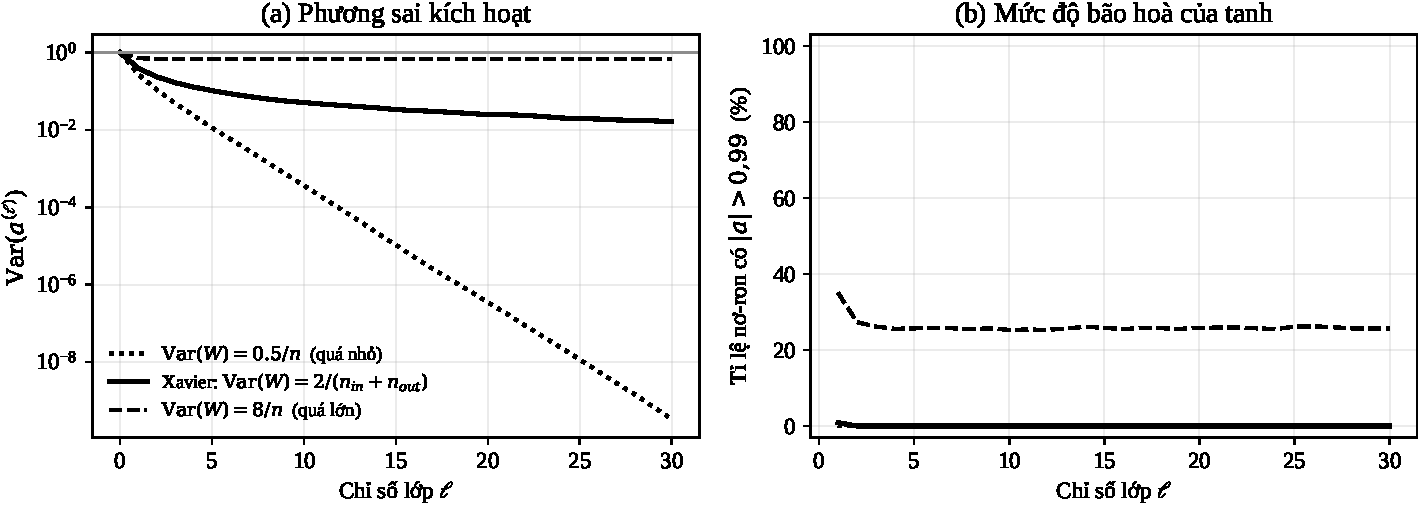
\includegraphics[width=0.98\textwidth]{Images/chap_2/hinh_khoitao.pdf}
\caption{Lan truyền tín hiệu xuôi qua $30$ lớp, mỗi lớp $256$ nơ-ron, kích hoạt
$\tanh$. (a) Phương sai kích hoạt theo thang log. Khi $\rho = 0{,}5 < 1$, phương
sai suy giảm theo cấp số nhân đúng như Hệ quả~\ref{hq:cap-so-nhan}; đường Xavier
($\rho = 1$) suy giảm chậm hơn hẳn, phù hợp quy luật điều hoà
\eqref{eq:dieu-hoa}. (b) Tỉ lệ nơ-ron bão hoà. Cấu hình $\rho = 8$ giữ được
phương sai chỉ nhờ $\tanh$ chặn giá trị, nhưng phải trả giá bằng khoảng $26\%$
nơ-ron rơi vào vùng $\sigma' \approx 0$.}
\label{fig:khoitao}
\end{figure}
 
\begin{figure}[H]
\centering
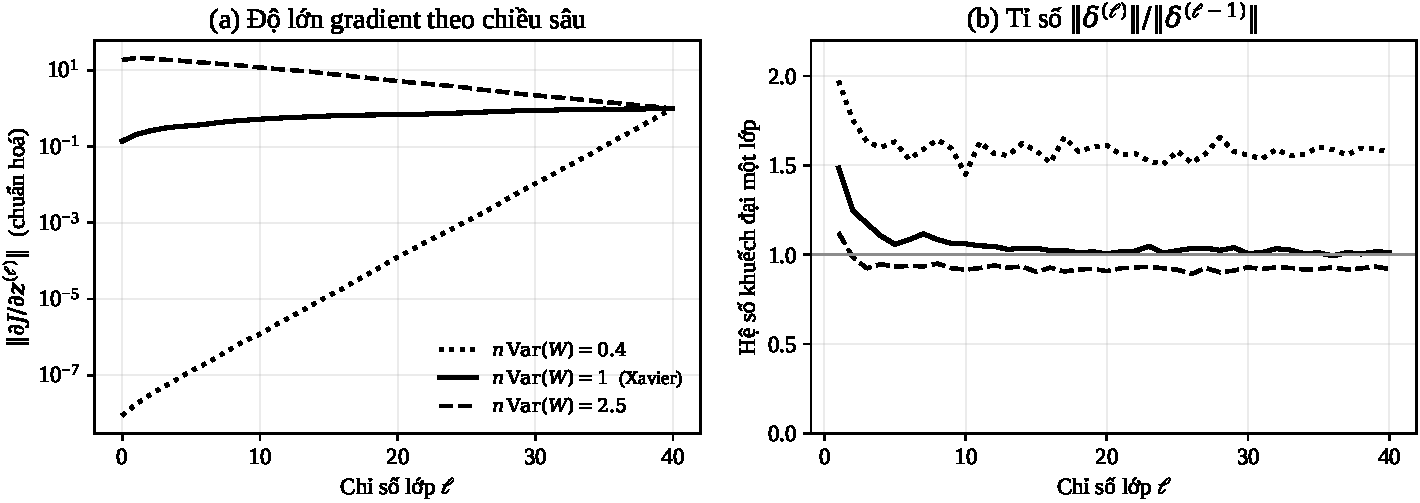
\includegraphics[width=0.98\textwidth]{Images/chap_2/hinh_gradient.pdf}
\caption{Lan truyền gradient ngược qua $40$ lớp, minh hoạ
Mệnh đề~\ref{md:tich-gradient}. (a) Chuẩn $\|\bm{\delta}^{(\ell)}\|$ theo thang
log: với $\rho = 0{,}4$, gradient tại lớp đầu nhỏ hơn tại lớp cuối khoảng $8$
bậc thập phân -- triệt tiêu gradient hoàn toàn. (b) Hệ số khuếch đại một lớp
$\|\bm{\delta}^{(\ell)}\|/\|\bm{\delta}^{(\ell-1)}\|$; đường Xavier bám sát mức
$1$, đúng như thiết kế của điều kiện \eqref{eq:dk-nguoc}.}
\label{fig:gradient}
\end{figure}
 
\begin{table}[H]
\centering
\caption{Kết quả thí nghiệm TN-C: mạng $12$ lớp, mỗi lớp $128$ nơ-ron, kích hoạt
$\tanh$, lô $N = 400$ mẫu chuẩn tắc. Cột ``bão hoà'' là tỉ lệ nơ-ron có
$|a^{(\ell)}| > 0{,}99$.}
\label{tab:so-lieu-khoitao}
\begin{tabular}{@{}c cc cc@{}}
\toprule
& \multicolumn{2}{c}{\textbf{Xavier}}
& \multicolumn{2}{c}{\textbf{Ngây thơ } $\mathcal{N}(0,1)$} \\
\cmidrule(lr){2-3}\cmidrule(lr){4-5}
$\ell$ & $\E[(a^{(\ell)})^2]$ & bão hoà & $\E[(a^{(\ell)})^2]$ & bão hoà \\
\midrule
1  & 0{,}391170 & 0{,}8\% & 0{,}929910 & 81{,}6\% \\
3  & 0{,}166306 & 0{,}0\% & 0{,}928834 & 81{,}0\% \\
5  & 0{,}105764 & 0{,}0\% & 0{,}927512 & 80{,}7\% \\
7  & 0{,}076834 & 0{,}0\% & 0{,}926659 & 80{,}8\% \\
9  & 0{,}060308 & 0{,}0\% & 0{,}928039 & 80{,}9\% \\
11 & 0{,}047046 & 0{,}0\% & 0{,}927819 & 80{,}8\% \\
\bottomrule
\end{tabular}
\end{table}
 
Bảng~\ref{tab:so-lieu-khoitao} làm rõ một điểm rất dễ bị hiểu sai. Nhìn riêng
cột phương sai, khởi tạo ngây thơ $\mathcal{N}(0,1)$ có vẻ ``ổn định'' hơn
Xavier vì $\E[(a^{(\ell)})^2]$ đứng yên quanh $0{,}93$ thay vì suy giảm. Nhưng
sự ổn định đó là giả tạo: theo Hệ quả~\ref{hq:cap-so-nhan} với
$\rho = n_{\text{in}}v = 128 \gg 1$, phương sai \emph{trước} kích hoạt bùng nổ
theo cấp số nhân, và chỉ bị $\tanh$ chặn cứng trong $(-1,1)$. Cái giá là $81\%$
nơ-ron nằm ngoài vùng $|a| \le 0{,}99$, nơi $\sigma' \approx 0$; theo
Mệnh đề~\ref{md:tich-gradient} gradient khi ấy bị triệt tiêu hoàn toàn. Bài học
phương pháp luận: \emph{phương sai kích hoạt một mình không phải chỉ báo đủ cho
sức khoẻ của mạng}; phải đọc kèm tỉ lệ bão hoà.
 
Bảng~\ref{tab:dieu-hoa} kiểm chứng trực tiếp dự đoán tiệm cận
\eqref{eq:dieu-hoa} của Mệnh đề~\ref{md:hieu-chinh}.
 
\begin{table}[H]
\centering
\caption{Kiểm chứng quy luật suy giảm điều hoà $s_\ell^2 \sim 1/(2\ell)$ cho
khởi tạo Xavier (số liệu cùng thí nghiệm TN-C).}
\label{tab:dieu-hoa}
\begin{tabular}{@{}c c c c@{}}
\toprule
$\ell$ & $s_\ell^2$ (thực nghiệm) & $1/(2\ell)$ (lý thuyết)
  & sai số tương đối \\
\midrule
1  & 0{,}391170 & 0{,}500000 & 21{,}8\% \\
3  & 0{,}166306 & 0{,}166667 & 0{,}2\% \\
5  & 0{,}105764 & 0{,}100000 & 5{,}8\% \\
7  & 0{,}076834 & 0{,}071429 & 7{,}6\% \\
9  & 0{,}060308 & 0{,}055556 & 8{,}6\% \\
11 & 0{,}047046 & 0{,}045455 & 3{,}5\% \\
\bottomrule
\end{tabular}
\end{table}
 
Sai lệch lớn tại $\ell = 1$ là điều dự kiến: \eqref{eq:dieu-hoa} là công thức
\emph{tiệm cận}, chỉ có hiệu lực khi $s_\ell^2$ đã đủ nhỏ để khai triển bậc hai
trong \eqref{eq:hieu-chinh} chiếm ưu thế. Từ $\ell \ge 3$ trở đi, sai số tương
đối giữ dưới $9\%$ trên toàn bộ dải khảo sát -- mức khớp chấp nhận được đối với
một công thức tiệm cận không chứa tham số tự do nào.

Hai dè dặt cần nêu để không đọc bảng quá mạnh. Thứ nhất, sai số tương đối
\emph{không đơn điệu} theo $\ell$ ($0{,}2\% \to 5{,}8\% \to 7{,}6\% \to 8{,}6\%
\to 3{,}5\%$), trong khi một công thức tiệm cận đúng phải cho sai số giảm dần;
dáng lên--xuống này đặc trưng cho nhiễu hữu hạn mẫu ở cỡ lô $N = 400$, và mức
khớp tại $\ell = 3$ có phần may mắn. Thứ hai, đẩy khai triển ở cuối chứng minh
thêm một bậc cho $u_\ell = 2\ell + \tfrac12\ln\ell + C + o(1)$, tức
$s_\ell^2$ phải nằm \emph{dưới} $1/(2\ell)$ với $\ell$ đủ lớn; số liệu tại
$\ell = 5,7,9$ lại nằm trên. Điều này không mâu thuẫn với
\eqref{eq:dieu-hoa} -- vốn chỉ khẳng định tỉ số tiến tới $1$ -- nhưng cho thấy
dải $\ell \le 11$ còn chịu ảnh hưởng của hằng số $C$ và của giai đoạn chuyển
tiếp. Muốn kiểm chứng chặt hơn cần tăng $N$ và mở rộng dải $\ell$.
 
\begin{nhanxet}[Giới hạn của kiểm chứng]
Cần nêu rõ phạm vi của kết luận trên. Số liệu ở Bảng~\ref{tab:dieu-hoa} thu được
từ một cấu hình duy nhất ($12$ lớp, $128$ nơ-ron, đầu vào chuẩn tắc) và tại thời
điểm khởi tạo, chưa qua huấn luyện. Nó kiểm chứng \emph{quy luật tiệm cận}
\eqref{eq:dieu-hoa}, không kiểm chứng rằng quy luật ấy còn đúng sau khi trọng số
đã được cập nhật -- điều mà không kết quả nào trong báo cáo khẳng định.
\end{nhanxet}
 
\subsection{Khởi tạo độ chệch và lựa chọn của báo cáo}
 
Độ chệch không gây vấn đề đối xứng một khi trọng số đã ngẫu nhiên: giả thiết
\eqref{eq:khoi-tao-hang} của Mệnh đề~\ref{md:doi-xung} đòi hỏi \emph{cả hai}
điều kiện đồng thời. Do đó quy ước $\bb^{(\ell)} = \bm{0}$ được sử dụng; quy ước
này cũng nhất quán với giả thiết (A2) của phân tích phương sai.
 
Tổng hợp Mục~\ref{sec:kichhoat} và Mục~\ref{sec:khoitao}, cấu hình áp dụng xuyên
suốt phần thực nghiệm của báo cáo là: hàm kích hoạt $\tanh$, khởi tạo Xavier
theo \eqref{eq:xavier}, độ chệch bằng $0$, lớp ra tuyến tính. Cấu hình
này đồng thời bảo đảm ba điều: (i) tính khả vi vô hạn cần cho toán tử vi phân
bậc hai, với mọi đạo hàm bị chặn đều (Bổ đề~\ref{bd:tanh-dao-ham} và
Hệ quả~\ref{hq:tanh-chan}); (ii) giữ $\bz^{(\ell)}$ trong vùng gần tuyến tính
của $\tanh$ tại thời điểm bắt đầu huấn luyện, tránh cái bẫy bão hoà được mô tả ở
Mệnh đề~\ref{md:tich-gradient}; (iii) cơ chế suy giảm phương sai theo chiều sâu
là đa thức chứ không phải mũ (Mệnh đề~\ref{md:hieu-chinh}).
 
%==============================================================================
\section{Lan truyền xuôi và hàm mục tiêu}
\label{sec:lantruyenxuoi}
%==============================================================================
 
\subsection{Thuật toán lan truyền xuôi}
 
\begin{algorithm}[H]
\caption{Lan truyền xuôi trên một lô dữ liệu}
\label{alg:forward}
\begin{algorithmic}[1]
\Require Lô $\bm{X} \in \R^{n_0 \times N}$; tham số
  $\btheta=\{\bW^{(\ell)},\bb^{(\ell)}\}_{\ell=1}^{L}$; hàm kích hoạt $\sigma$
\Ensure Đầu ra $\bm{Y} \in \R^{n_L \times N}$ và các kích hoạt trung gian
  $\{\bm{Z}^{(\ell)},\bm{A}^{(\ell)}\}$
\State $\bm{A}^{(0)} \gets \bm{X}$
\For{$\ell = 1$ \textbf{đến} $L$}
  \State $\bm{Z}^{(\ell)} \gets \bW^{(\ell)}\bm{A}^{(\ell-1)}
          + \bb^{(\ell)}\bm{1}_N^{\top}$
    \Comment{\eqref{eq:batch}}
  \If{$\ell < L$}
    \State $\bm{A}^{(\ell)} \gets \sigma\!\left(\bm{Z}^{(\ell)}\right)$
  \Else
    \State $\bm{A}^{(L)} \gets \bm{Z}^{(L)}$
      \Comment{lớp ra tuyến tính, theo \eqref{eq:fnn-output}}
  \EndIf
  \State lưu $\bm{Z}^{(\ell)}, \bm{A}^{(\ell)}$ vào đồ thị tính toán
\EndFor
\State \Return $\bm{Y} \gets \bm{A}^{(L)}$
\end{algorithmic}
\end{algorithm}
 
Bước lưu trữ ở dòng 9 không phải chi tiết kỹ thuật phụ: chính các giá trị trung
gian này tạo thành \emph{đồ thị tính toán} mà vi phân tự động sẽ duyệt ngược để
tính $\nabla_{\btheta} J$ (Chương~\ref{chap:autodiff}). Chi phí bộ nhớ tương ứng
đã được nêu ở Mệnh đề~\ref{md:chi-phi}, và nó là lý do vì sao trong bài toán
PINN, số điểm phối trí $N$ bị giới hạn bởi bộ nhớ chứ không bởi thời gian tính.
 
Thí nghiệm TN-A xác nhận tính đúng đắn của cài đặt trên kiến trúc $(2,4,4,1)$ với
lô $N = 5$: hình dạng tensor biến đổi theo đúng
$\bm{A}^{(0)} \in \R^{2\times5} \to \bm{A}^{(1)},\bm{A}^{(2)} \in \R^{4\times5}
\to \bm{A}^{(3)} \in \R^{1\times5}$, và số tham số đếm được đúng bằng $37$ như
\eqref{eq:so-tham-so} dự đoán (xem Hình~\ref{fig:kien-truc-fnn}).
 
\subsection{Cơ sở xác suất của hàm mục tiêu}
\label{subsec:ham-muc-tieu}
 
Theo Mục 6.2 của Goodfellow và cộng sự~\cite{goodfellow2016}, cách tiếp cận hiện
đại không định nghĩa hàm mất mát một cách tuỳ ý mà suy ra nó từ nguyên lý
\emph{hợp lý cực đại}. Giả sử mạng tham số hoá một phân phối có điều kiện
$p_{\text{model}}(\bm{y}\mid\bx;\btheta)$ và dữ liệu được lấy mẫu từ phân phối
thực nghiệm $\hat{p}_{\text{data}}$. Ước lượng hợp lý cực đại tương đương với
cực tiểu hoá đối log-hợp lý âm:
\begin{equation}
J(\btheta)
 = -\,\E_{(\bx,\bm{y}) \sim \hat{p}_{\text{data}}}
   \left[ \log p_{\text{model}}(\bm{y}\mid\bx;\btheta) \right].
\label{eq:nll}
\end{equation}
 
\begin{menhde}[Hồi quy Gauss sinh ra MSE]
\label{md:gauss-mse}
Chọn
\[
  p_{\text{model}}(\bm{y}\mid\bx;\btheta)
  = \mathcal{N}\!\big(\bm{y};\, \Net_{\btheta}(\bx),\,
    \varsigma^{2}\bI_{n_L}\big),
\]
với $\varsigma > 0$ cố định. Khi đó
\begin{equation}
J(\btheta)
 = \frac{1}{2\varsigma^{2}}\,
   \E_{\hat{p}_{\text{data}}}
   \big\| \bm{y} - \Net_{\btheta}(\bx) \big\|_2^{2}
   + \frac{n_L}{2}\log\!\big(2\pi\varsigma^2\big),
\label{eq:mse}
\end{equation}
trong đó số hạng thứ hai không phụ thuộc $\btheta$. Do đó cực tiểu hoá
\eqref{eq:nll} tương đương với cực tiểu hoá sai số bình phương trung bình.
\end{menhde}
 
\begin{proof}
Mật độ Gauss nhiều chiều với ma trận hiệp phương sai $\varsigma^2\bI$ là
\[
p(\bm{y}\mid\bx) = \big(2\pi\varsigma^2\big)^{-n_L/2}
  \exp\!\left(-\frac{\|\bm{y} - \Net_{\btheta}(\bx)\|_2^2}{2\varsigma^2}\right).
\]
Lấy logarit và đổi dấu:
$-\log p = \frac{\|\bm{y} - \Net_{\btheta}(\bx)\|_2^2}{2\varsigma^2}
+ \frac{n_L}{2}\log(2\pi\varsigma^2)$. Lấy kỳ vọng theo
$\hat p_{\text{data}}$ cho \eqref{eq:mse}. Vì $\varsigma$ cố định, hai bài toán
cực tiểu hoá có cùng tập nghiệm.
\end{proof}
 
Nói cách khác, MSE không phải một lựa chọn tuỳ tiện mà là hệ quả trực tiếp của
giả thiết nhiễu Gauss đồng phương sai. Mệnh đề sau xác định mục tiêu lý tưởng mà
việc cực tiểu hoá ấy hướng tới, và tách sai số thành hai phần có bản chất khác
nhau.
 
\begin{menhde}[Nghiệm tối ưu của MSE là kỳ vọng có điều kiện]
\label{md:ky-vong-dieu-kien}
Trong lớp mọi hàm đo được $g$ với $\E\|g(\bx)\|^2 < \infty$, phiếm hàm
$g \mapsto \E\big[\|\bm{y} - g(\bx)\|_2^2\big]$ đạt cực tiểu tại
$g^{*}(\bx) = \E[\bm{y} \mid \bx]$, và
\begin{equation}
\E\big[\|\bm{y} - g(\bx)\|^2\big]
 = \underbrace{\E\big[\|\bm{y} - g^{*}(\bx)\|^2\big]}_{\text{nhiễu không khử
   được}}
 + \E\big[\|g^{*}(\bx) - g(\bx)\|^2\big].
\label{eq:phan-tich-mse}
\end{equation}
\end{menhde}
 
\begin{proof}
Viết $\bm{y} - g(\bx) = \big(\bm{y} - g^{*}(\bx)\big) + \big(g^{*}(\bx) -
g(\bx)\big)$ và khai triển bình phương. Số hạng chéo là
\[
2\,\E\Big[\big\langle \bm{y} - g^{*}(\bx),\; g^{*}(\bx) - g(\bx)\big\rangle\Big]
= 2\,\E\Big[\big\langle \E[\bm{y} - g^{*}(\bx)\mid\bx],\;
   g^{*}(\bx) - g(\bx)\big\rangle\Big] = 0,
\]
trong đó bước đầu dùng luật kỳ vọng lặp (hợp lệ vì $g^{*}(\bx)-g(\bx)$ đo được
theo $\bx$), bước sau dùng $\E[\bm{y}\mid\bx] = g^{*}(\bx)$. Ta được
\eqref{eq:phan-tich-mse}; vế phải cực tiểu khi và chỉ khi số hạng thứ hai bằng
$0$, tức $g = g^{*}$ hầu chắc chắn.
\end{proof}
 
\begin{nhanxet}[Vì sao phân tích này thay đổi khi chuyển sang phần dư]
Trong bài toán phương trình vi phân, số hạng ``nhiễu không khử được'' trong
\eqref{eq:phan-tich-mse} biến mất: phần dư được đánh giá bằng chính phương trình
chứ không bằng dữ liệu đo có nhiễu, nên tồn tại hàm làm hàm mục tiêu bằng đúng
$0$ (chính là nghiệm đúng, nếu nó thuộc lớp hàm biểu diễn được). Hệ quả là mọi
sai số quan sát được trong thực nghiệm PINN đều thuộc về một trong ba nguồn: sai
số xấp xỉ (lớp hàm không chứa nghiệm), sai số tối ưu (thuật toán không tìm được
điểm cực tiểu), và sai số rời rạc hoá (tập điểm phối trí hữu hạn). Việc phân tách
ba nguồn này là nội dung của phần đánh giá số ở
Chương~\ref{chap:thucnghiem}.
\end{nhanxet}
 
\subsection{Tính không lồi của hàm mục tiêu}
 
\begin{menhde}[Đối xứng dấu kéo theo không lồi]
\label{md:khong-loi}
Xét mạng một lớp ẩn với $\sigma$ lẻ (chẳng hạn $\tanh$),
$\Net_{\btheta}(\bx) = \bW^{(2)}\sigma\big(\bW^{(1)}\bx + \bb^{(1)}\big)
+ \bb^{(2)}$, và $J$ là hàm mục tiêu MSE \eqref{eq:mse}. Đặt
\begin{equation}
\btheta = \big(\bW^{(1)}, \bb^{(1)}, \bW^{(2)}, \bb^{(2)}\big),
\qquad
\btheta^{-} := \big(-\bW^{(1)}, -\bb^{(1)}, -\bW^{(2)}, \bb^{(2)}\big).
\label{eq:doi-xung-dau}
\end{equation}
Khi đó $\Net_{\btheta} \equiv \Net_{\btheta^{-}}$, nên
$J(\btheta) = J(\btheta^{-})$. Nếu tồn tại $\btheta$ với
$J(\btheta) < J\big(\tfrac{1}{2}(\btheta + \btheta^{-})\big)$ thì $J$
\emph{không lồi} trên $\R^P$.
\end{menhde}
 
\begin{proof}
Vì $\sigma$ lẻ,
$\sigma\big(-\bW^{(1)}\bx - \bb^{(1)}\big)
 = -\sigma\big(\bW^{(1)}\bx + \bb^{(1)}\big)$, nên
\[
\Net_{\btheta^{-}}(\bx)
 = \big(-\bW^{(2)}\big)\Big(-\sigma\big(\bW^{(1)}\bx+\bb^{(1)}\big)\Big)
   + \bb^{(2)} = \Net_{\btheta}(\bx).
\]
Vì $J$ chỉ phụ thuộc $\btheta$ thông qua hàm $\Net_{\btheta}$, ta có
$J(\btheta) = J(\btheta^{-})$.
 
Trung điểm là $\bar{\btheta} := \tfrac12(\btheta + \btheta^{-})
 = \big(\bm{0},\bm{0},\bm{0},\bb^{(2)}\big)$, ứng với hàm hằng
$\Net_{\bar{\btheta}} \equiv \bb^{(2)}$. Nếu $J$ lồi thì
\[
J(\bar{\btheta}) \le \tfrac12 J(\btheta) + \tfrac12 J(\btheta^{-})
 = J(\btheta),
\]
mâu thuẫn với giả thiết $J(\btheta) < J(\bar\btheta)$.
\end{proof}
 
\begin{nhanxet}
\label{nx:doi-xung-hoan-vi}
Giả thiết trong Mệnh đề~\ref{md:khong-loi} hầu như luôn được thoả trong thực tế:
nó chỉ đòi hỏi tồn tại \emph{một} bộ tham số cho sai số nhỏ hơn mô hình hằng tốt
nhất -- điều hiển nhiên đúng với bất kỳ tập dữ liệu không tầm thường nào.
 
Bên cạnh đối xứng dấu, mạng còn có \emph{đối xứng hoán vị}: với mọi hoán vị
$\pi$ của $\{1,\dots,n_1\}$, việc hoán vị đồng thời các hàng của
$\bW^{(1)}, \bb^{(1)}$ và các cột của $\bW^{(2)}$ giữ nguyên hàm được biểu diễn.
Kết hợp hai loại đối xứng, mỗi điểm cực tiểu ``bản chất'' sinh ra ít nhất
$2^{n_1}\, n_1!$ điểm cực tiểu trong không gian tham số. Với $n_1 = 20$, con số
này đã vượt $10^{24}$.
 
Bức tranh này -- không lồi, đối xứng phong phú, vô số cực tiểu tương đương -- là
lý do các bảo đảm hội tụ toàn cục vắng bóng trong toàn bộ lĩnh vực, và là lý do
phương pháp luận thực nghiệm của báo cáo phải dựa trên nhiều lần chạy với hạt
giống ngẫu nhiên khác nhau, báo cáo cả trung bình lẫn độ phân tán, thay vì một
lần chạy duy nhất. Một kết quả tốt từ một hạt giống may mắn không phải là bằng
chứng về phương pháp.
\end{nhanxet}
 
\subsection{Cầu nối sang bài toán phương trình vi phân}
 
\begin{nhanxet}[Từ MSE tới phần dư]
\label{nx:cau-noi}
Trong khuôn khổ giải phương trình vi phân bằng mạng nơ-ron, ta không có sẵn cặp
$(\bx_i,\bm{y}_i)$ với $\bm{y}_i$ là nghiệm đúng. Thay vào đó, ``nhãn'' được
thay bằng \emph{phần dư} của phương trình: với toán tử vi phân $\mathcal{L}$, vế
phải $f$ và điều kiện biên $g$, ta cực tiểu hoá
\begin{equation}
J(\btheta)
 = \frac{1}{N_r}\sum_{i=1}^{N_r}
   \big| \mathcal{L}\big[\Net_{\btheta}\big](\bx_i) - f(\bx_i) \big|^{2}
 + \lambda\,\frac{1}{N_b}\sum_{j=1}^{N_b}
   \big| \Net_{\btheta}(\bx_j) - g(\bx_j) \big|^{2}.
\label{eq:pinn-loss}
\end{equation}
Cấu trúc của \eqref{eq:pinn-loss} vẫn là MSE như \eqref{eq:mse}; ba điểm khác
biệt, mỗi điểm mở ra một mục của các chương sau.
 
Thứ nhất, sự xuất hiện của $\mathcal{L}[\Net_{\btheta}]$ đòi hỏi đạo hàm của
mạng theo \emph{biến đầu vào} -- tức chính các đại lượng được cho tường minh bởi
Mệnh đề~\ref{md:jacobian} và Mệnh đề~\ref{md:hessian}, và được tính hiệu quả
bằng vi phân tự động ở Chương~\ref{chap:autodiff}.
Hệ quả~\ref{hq:pinn-hong} cho thấy điều gì xảy ra khi các đại lượng ấy đồng nhất
triệt tiêu.
 
Thứ hai, hàm mục tiêu là tổng của hai số hạng có \emph{thứ nguyên khác nhau} --
phần dư mang thứ nguyên của $\mathcal{L}u$, còn số hạng biên mang thứ nguyên của
$u$ -- nên hệ số $\lambda$ không phải một siêu tham số tuỳ chọn mà là một đại
lượng cần được xác định. Đây là bài toán cân bằng trọng số mất mát, được phân
tích ở Chương~\ref{chap:pinn}.
 
Thứ ba, tập điểm $\{\bx_i\}$ không phải dữ liệu quan sát mà do người dùng
\emph{chọn}. Số lượng và phân bố của chúng trở thành tham số thiết kế, tương tự
vai trò của lưới trong phương pháp số cổ điển, nhưng không chịu ràng buộc về
tính chính quy của lưới.
\end{nhanxet}
 
%==============================================================================
\section*{Kết luận chương}
\addcontentsline{toc}{section}{Kết luận chương}
%==============================================================================
 
Chương này đã thiết lập các kết quả nền tảng cho phần còn lại của báo cáo, được
tổng hợp trong Bảng~\ref{tab:tong-ket}. Điểm chung của chúng: mỗi lựa chọn thiết
kế trong phần thực nghiệm đều truy về được một mệnh đề cụ thể, chứ không về một
quy ước thực hành.
 
\begingroup
\small
\setlength{\LTcapwidth}{\textwidth}
\begin{longtable}{@{}l p{8.2cm}@{}}
\caption{Tổng kết các kết quả chính của chương và vai trò của chúng.}
\label{tab:tong-ket} \\
\toprule
\textbf{Kết quả} & \textbf{Nội dung và vai trò} \\
\midrule
\endfirsthead
\multicolumn{2}{@{}l}{\emph{Bảng~\thetable{} (tiếp theo)}} \\
\toprule
\textbf{Kết quả} & \textbf{Nội dung và vai trò} \\
\midrule
\endhead
\midrule
\multicolumn{2}{r@{}}{\emph{(xem tiếp trang sau)}} \\
\endfoot
\bottomrule
\endlastfoot
Bổ đề~\ref{bd:affine}, Hệ quả~\ref{hq:suy-bien}
  & Hợp thành affine vẫn affine; phi tuyến là nguồn duy nhất của sức biểu
    diễn. \\
Mệnh đề~\ref{md:chi-phi}
  & Chi phí lan truyền xuôi $2N\sum_\ell n_\ell n_{\ell-1}$: tuyến tính theo số
    điểm, bậc hai theo bề rộng. \\
Mệnh đề~\ref{md:jacobian}, \ref{md:hessian}
  & Công thức truy hồi cho Jacobian và Hessian theo biến đầu vào -- công cụ
    trung tâm cho mọi tính toán phần dư (Thuật toán~\ref{alg:dao-ham}). \\
Hệ quả~\ref{hq:relu-hessian}
  & $\sigma'' \equiv 0 \Rightarrow \nabla^2_{\bx}\Net = 0$: tiêu chuẩn loại trừ
    hàm kích hoạt. \\
Mệnh đề~\ref{md:xor-chan-duoi}
  & Chặn dưới $J \ge \tfrac14$ cho mọi mô hình affine trên XOR, chứng minh bằng
    bất biến trung điểm. \\
Định lý~\ref{dl:xap-xi}, \ref{dl:sobolev}
  & Trù mật trong $C(K)$ khi và chỉ khi $\sigma$ không đa thức; trù mật trong
    $C^k(K)$ -- cơ sở lý thuyết cho phương pháp. \\
Định lý~\ref{dl:barron}
  & Tốc độ $\mathcal{O}(m^{-1/2})$ không phụ thuộc số chiều; lập luận định
    hướng chống lời nguyền số chiều. \\
Mệnh đề~\ref{md:da-thuc}
  & Hàm kích hoạt đa thức cho lớp hàm hữu hạn chiều, không trù mật. \\
Bổ đề~\ref{bd:tanh-dao-ham}, Hệ quả~\ref{hq:tanh-chan}
  & $\tanh^{(k)} = P_k(\tanh)$ với $\deg P_k = k+1$; mọi đạo hàm bị chặn đều. \\
Định lý~\ref{dl:relu-tuyen-tinh}, Mệnh đề~\ref{md:dirac}
  & Mạng ReLU tuyến tính từng khúc; đạo hàm bậc hai là tổ hợp độ đo Dirac. \\
Hệ quả~\ref{hq:pinn-hong}
  & Với ReLU, hàm mục tiêu phần dư là \emph{hằng số địa phương}: mọi thuật toán
    gradient đứng yên tuyệt đối. \\
Mệnh đề~\ref{md:tich-gradient}
  & Chặn mũ $\sech^{2(L-1)}(\tau)$ cho gradient khi bão hoà. \\
Mệnh đề~\ref{md:doi-xung}, Nhận xét~\ref{nx:phan-vi-du}
  & Khởi tạo hằng giữ nguyên đối xứng hoán vị; giả thiết ``các hàng bằng nhau''
    là không đủ. \\
Mệnh đề~\ref{md:var-xuoi}--\ref{md:var-nguoc}, \eqref{eq:xavier}, \eqref{eq:he}
  & Điều kiện bảo toàn phương sai xuôi/ngược; công thức Xavier và He. \\
Mệnh đề~\ref{md:hieu-chinh}
  & Hiệu chỉnh bậc hai: $s_\ell^2 \sim 1/(2\ell)$, suy giảm điều hoà chứ không
    mũ; khớp thực nghiệm với sai số $< 9\%$ từ $\ell \ge 3$. \\
Mệnh đề~\ref{md:gauss-mse}, \ref{md:ky-vong-dieu-kien}
  & MSE sinh từ hợp lý cực đại; nghiệm lý tưởng là $\E[\bm{y}\mid\bx]$. \\
Mệnh đề~\ref{md:khong-loi}
  & $J$ không lồi do đối xứng dấu; ít nhất $2^{n_1}n_1!$ cực tiểu tương đương.
\end{longtable}
\endgroup
 
Cấu hình được chốt lại cho toàn bộ phần thực nghiệm: kiến trúc FNN với hàm kích
hoạt $\tanh$, khởi tạo Xavier theo \eqref{eq:xavier}, độ chệch bằng $0$,
lớp ra tuyến tính. Mỗi thành phần của cấu hình này được biện minh bởi ít nhất
một kết quả trong Bảng~\ref{tab:tong-ket}.
 
Chương này cũng đã xác định rõ biên giới của những gì đã chứng minh được. Các
định lý xấp xỉ phổ quát bảo đảm sự \emph{tồn tại} của một bộ tham số tốt;
Mệnh đề~\ref{md:khong-loi} cho thấy không có bảo đảm nào rằng thuật toán tối ưu
sẽ tìm ra nó. Khoảng cách giữa hai điều đó chính là lý do phần đánh giá số của
báo cáo là bắt buộc chứ không phải minh hoạ.
 
Chương tiếp theo trình bày cơ chế tính $\nabla_{\btheta} J$ và các đạo hàm theo
biến đầu vào bằng vi phân tự động -- công cụ hiện thực hoá các công thức truy hồi
\eqref{eq:G-truy-hoi} và \eqref{eq:S-truy-hoi} một cách hiệu quả và không cần
viết tường minh $\sigma''$ -- cùng các thuật toán tối ưu tương ứng.
 